



\section{Deterministic Inference Encourages Benchmark Memorization}
\label{sec:glue-memorization}

The previous section argued that \textbf{bitwise-deterministic inference} is not a natural
primitive for \textbf{probabilistic generative models}. We now show that, even at the
\emph{evaluation} level, insisting on a single deterministic output per input risks
repeating an old mistake from the pre-LLM era: the \textbf{GLUE saturation story}.
Our claim in this section is simple:

%\begin{quote}
%  \emph{Deterministic inference---``one input, one canonical output, one scalar
%  score''---encourages models to memorize benchmark surfaces rather than to  genuinely generalize.}
%\end{quote}

We first revisit GLUE as a cautionary tale of \textbf{single-score benchmark culture},
then show how modern \textbf{sequence-level deterministic inference} is structurally
analogous. Finally, we introduce a GLUE-style robustness protocol over four LLM
families and construct a \textbf{heatmap of robustness} that directly visualizes
the cost of determinism.

\begin{tcolorbox}[colback=gray!5,colframe=black!60,sharp corners]
\textbf{Claim 1}:
\textbf{Deterministic inference—``one input, one canonical output, one scalar score''—turns evaluation into answer–from–memory:} success is measured by reproducing a fixed surface form, not how stably the model supports a distribution of semantically correct responses.
\end{tcolorbox}


\subsection{GLUE as a Cautionary Tale}
\label{subsec:glue-history}

The \textbf{GLUE benchmark}~\cite{wang2018glue} was designed as a multi-task testbed
for natural language understanding, aggregating performance across nine tasks,
including natural language inference (MNLI, RTE), paraphrase detection (QQP),
question answering (QNLI), and sentiment analysis (SST-2). GLUE was an enormous
success: it provided a standardized evaluation suite and a single scalar ``GLUE
score'' that made progress easy to track and compare. SuperGLUE extended this
template with harder tasks and an even more entrenched leaderboard culture
\cite{wang2019glue}.

GLUE's design implicitly enshrined a particular notion of performance:
for each example $(x_i, y_i)$ and model $f_\theta$, the evaluation pipeline
asked for a \emph{single predicted label} $\hat{y}_i = f_\theta(x_i)$ and
computed an accuracy or $F_1$ score by comparing $\hat{y}_i$ to $y_i$.
The whole community then reported a \textbf{single scalar}:
\[
  \text{GLUEScore}(f_\theta) \;=\; \frac{1}{T} \sum_{t=1}^T \text{Acc}_t(f_\theta)\,,
\]
where $t$ indexes tasks. There was no notion of \emph{distribution over
predictions}, \emph{uncertainty}, or \emph{robustness}; only a single
deterministic mapping from inputs to labels.

Within roughly two years, GLUE was effectively ``solved'':
state-of-the-art models reported scores at or above estimated human
performance. Yet follow-up work revealed that these impressive numbers
often reflected \textbf{shortcut learning} rather than deep understanding.
Gururangan et al.\ and others documented pervasive annotation artifacts
and label biases in NLI and related tasks~\cite{gururangan2018annotation,mccoy2019right}.
Geirhos et al.\ showed more broadly how deep networks, given a fixed benchmark,
gravitate toward \emph{cheap, brittle heuristics} that exploit spurious
correlations~\cite{geirhos2020shortcut}. Counterfactually augmented data,
checklist-style tests, and adversarial GLUE variants further exposed how
modest perturbations, paraphrases, or distribution shifts caused sharp
performance drops despite near-perfect leaderboard scores
\cite{kaushik2020learning,ribeiro2020checklist,wang2021adversarialglue,chen2021mandoline,yuan2023revisiting}.

From a statistical perspective, the problem is not that GLUE was ``bad'',
but that the combination of \textbf{finite test sets} and \textbf{single-output
evaluation} creates an \emph{evaluation surface} that can be memorized.
Once models and training pipelines are tuned directly against that surface,
new parameters are free to overfit the idiosyncrasies of the benchmark's
finite sample. The resulting leaderboards give an illusion of steady
progress even as out-of-distribution behavior stagnates.

\subsection{From Label Determinism to Sequence Determinism}
\label{subsec:sequence-determinism}

Large language models extend this picture in two important ways:
they are \emph{generative}, and they are \emph{stochastic}. Instead of
learning a classifier $f_\theta(x) \rightarrow y$, they learn a conditional
distribution
\[
  p_\theta(y \mid x)\,,
\]
where $y$ is a \emph{text sequence}, not a single label. Evaluation,
however, often collapses this distribution back into a deterministic
mapping by choosing a fixed decoding strategy
$\text{Dec}_d\colon p_\theta(\cdot \mid x) \mapsto \hat{y}$.
For example, a \textbf{greedy $T{=}0$ decoder} defines
\[
  \hat{y}^{\text{det}}(x) \;=\;
  \text{Dec}_{\text{greedy}}(p_\theta(\cdot \mid x))
  \;=\; \arg\max_{y} p_\theta(y \mid x)\,,
\]
where in practice the argmax is taken token by token.

In many contemporary LLM evaluations, especially those adapted from
GLUE-style tasks, performance is reported as
\[
  \text{Acc}^{\text{det}}(f_\theta) \;=\;
  \frac{1}{N} \sum_{i=1}^N
  \mathbb{1}\bigl[\phi(\hat{y}^{\text{det}}(x_i)) = y_i\bigr]\,,
\]
where $\phi$ extracts a label (e.g., a multiple-choice option) from the
deterministic completion. This is \emph{structurally identical} to the
original GLUE protocol: one input, one output, one bit of correctness.

Yet, from the standpoint of \textbf{artificial cognition}, the meaningful
object is not $\hat{y}^{\text{det}}(x)$ but the \emph{entire distribution}
$p_\theta(y \mid x)$. Different decoding strategies---temperature sampling,
nucleus sampling, self-consistency, Tree-of-Thought---all probe different
slices of this distribution and often reveal capabilities that deterministic
greedy decoding hides~\cite{holtzman2020degeneration,wang2022selfconsistency,yao2023treeofthought}.
Insisting on a single deterministic trace amounts to replaying the GLUE
error at the sequence level: \textbf{we optimize and evaluate against a
single surface point on a much richer distribution}.

To make this concern concrete, we now design a GLUE-style robustness
protocol over four widely used tasks and a diverse set of LLM families,
explicitly contrasting deterministic vs.\ stochastic evaluation.

\subsection{Experimental Setup: GLUE-Style Robustness Under Decoding Choices}
\label{subsec:glue-setup}

\paragraph{Tasks.}
We focus on four GLUE tasks that are both influential and amenable to
paraphrastic manipulation:

\begin{itemize}[leftmargin=1.5em]
  \item \textbf{MNLI} (Multi-Genre Natural Language Inference): three-way
        classification (entailment, contradiction, neutral) over
        premise--hypothesis pairs with diverse genres.
  \item \textbf{QQP} (Quora Question Pairs): binary paraphrase detection
        over question pairs; especially susceptible to lexical overlap
        shortcuts.
  \item \textbf{QNLI}: question--sentence pairs derived from SQuAD;
        recast as binary entailment, testing whether a sentence
        answers a question.
  \item \textbf{SST-2}: binary sentiment classification at the
        sentence level.
\end{itemize}

For each task $t \in \{\text{MNLI},\text{QQP},\text{QNLI},\text{SST-2}\}$,
we start from a held-out test (or dev) set
\[
  \mathcal{D}_t^{\text{orig}} 
  \;=\; \{(x_i^{(t)}, y_i^{(t)})\}_{i=1}^{N_t}\,,
\]
where $x_i^{(t)}$ is the input text (single sentence or pair) and
$y_i^{(t)}$ is the gold label.

\paragraph{Paraphrastic and perturbed variants.}
To probe generalization beyond the benchmark surface, we create three
additional variants for each task:

\begin{itemize}[leftmargin=1.5em]
  \item \textbf{Paraphrased} ($\mathcal{D}_t^{\text{para}}$): for each
        example, we generate 2--3 paraphrastic rewrites of one or both
        segments (premise/hypothesis, question/sentence) using a strong
        paraphrase model and filter them to preserve the label; e.g.,
        by requiring high entailment confidence or human verification.
  \item \textbf{Perturbed} ($\mathcal{D}_t^{\text{pert}}$): we apply
        small lexical and syntactic transformations that should not
        change the label: synonym substitution, tense changes,
        active/passive alternation, or mild word-order shuffles.
  \item \textbf{Adversarial paraphrased} ($\mathcal{D}_t^{\text{adv}}$):
        we prompt an LLM to produce label-preserving but challenging
        rewrites (e.g., ``keep the answer label unchanged but attempt to
        confuse a classifier by changing connectives and information
        order''), again filtered for correctness.
\end{itemize}

Each variant shares the same labels $y_i^{(t)}$ but differs in surface
form. Together, these sets allow us to distinguish \textbf{surface
memorization} from \textbf{semantic robustness}.

\paragraph{Models.}
To connect with our FRACTURE analysis, we evaluate the same
\textbf{17-model zoo} used in Figure~\ref{fig:fracture-heatmap}:

\begin{center}
\small
LLaMA-2 7B,
LLaMA-2 13B,
Vicuna-7B,
LLaMA-3 8B,
Gemma~2 9B,
Gemma~2 27B,
Mistral-7B,
Mixtral-8$\times$7B,
Phi-2,
LLaMA-3 7B,
LLaMA-3 70B,
Claude,
Mixtral-8$\times$22B,
GPT-3.5,
GPT-4o,
GPT-4o mini,
DeepSeek.
\end{center}



These span open and closed models, small and large scales, and a variety
of training pipelines. For each model $m$ we use its official
instruction-tuned checkpoint and recommended prompting style.

\paragraph{Decoding modes.}
For each model $m$ and task $t$, we define two decoding modes:

\begin{itemize}[leftmargin=1.5em]
  \item \textbf{Deterministic} (\emph{Det}): temperature $T = 0$,
        greedy decoding, nucleus $p = 1.0$ (i.e., no sampling).
        This corresponds to the ``deterministic inference'' advocated
        by batch-invariant kernel designs~\cite{he2025defeating}.
  \item \textbf{Stochastic} (\emph{Stoch}): moderate temperature
        and nucleus sampling, e.g.\ $T = 0.7$, top-$p = 0.9$,
        with $K$ independent samples per input (we use $K = 10$).
\end{itemize}

In both modes, we prompt the model with a natural-language description
of the task and a constrained answer format (e.g., options A/B/C).
A deterministic \emph{label-extraction function} $\phi$ maps each
completion into a label in the task's label set.

\paragraph{Deterministic vs.~distributional evaluation.}
For each task $t$, dataset variant $v \in \{\text{orig},\text{para},
\text{pert},\text{adv}\}$, model $m$, and decoding mode $d$, we compute
\emph{per-split accuracies} as follows.

\begin{itemize}[leftmargin=1.5em]
  \item \textbf{Deterministic accuracy.} In Det mode, we generate a
        single completion $\hat{y}^{\text{det}}$ for each input and
        compute
        \[
          A_{t,v}^{\text{det}}(m)
          \;=\;
          \frac{1}{|\mathcal{D}_t^{v}|}
          \sum_{(x,y) \in \mathcal{D}_t^{v}}
          \mathbb{1}\!\bigl[\phi(\hat{y}^{\text{det}}(x)) = y\bigr]\,.
        \]
  \item \textbf{Stochastic majority-vote accuracy.} In Stoch mode,
        we draw $K$ independent completions
        $\hat{y}^{(1)}, \dots, \hat{y}^{(K)}$ and take a
        \emph{majority-vote label}
        \[
          \tilde{y}(x) \;=\;
          \text{mode}\bigl(\phi(\hat{y}^{(1)}(x)), \dots,
                           \phi(\hat{y}^{(K)}(x))\bigr)\,.
        \]
        We then compute
        \[
          A_{t,v}^{\text{stoch}}(m)
          \;=\;
          \frac{1}{|\mathcal{D}_t^{v}|}
          \sum_{(x,y) \in \mathcal{D}_t^{v}}
          \mathbb{1}\!\bigl[\tilde{y}(x) = y\bigr]\,.
        \]
        This treats the model as a \emph{distribution over labels} and
        asks whether the \emph{mode} of that distribution is correct.
\end{itemize}

We further record, for analysis but not for the heatmap, per-example
\emph{label entropy} and \emph{disagreement rate} across samples, which
quantify the model's epistemic uncertainty~\cite{atil2024stability}.

\paragraph{A robustness ratio.}
To isolate robustness rather than absolute accuracy, we define a
\emph{GLUE robustness ratio} for each triplet $(t,m,d)$:
\[\boxed{
  R_t^{(d)}(m)
  \;=\;
  \frac{
    A_{t,\text{para}}^{(d)}(m)
    + A_{t,\text{pert}}^{(d)}(m)
    + A_{t,\text{adv}}^{(d)}(m)
  }{
    3 \, A_{t,\text{orig}}^{(d)}(m)
  }\,.
  }
\]
By construction, $R_t^{(d)}(m) \in [0,1]$ whenever the model performs
no better on the variants than on the original split. A value near
$1$ indicates that \emph{performance on paraphrased, perturbed, and
adversarially rewritten inputs matches performance on the original
benchmark surface}. A value substantially below $1$ indicates that
the model's high GLUE score is \emph{not robust}: it collapses under
simple rephrasings of the same underlying semantics.

This normalization is important. Models differ in absolute strength:
a small student model may have lower raw accuracy but a higher
\emph{robustness ratio} than a large SOTA model. By focusing on
$R_t^{(d)}(m)$, we explicitly separate \textbf{competence}
(high $A_{t,\text{orig}}$) from \textbf{generalization}
(high $R_t^{(d)}$), and we can ask how \emph{decoding choices} affect
the latter.

\subsection{A GLUE Robustness Heatmap for Deterministic vs.~Stochastic Inference}
\label{subsec:glue-heatmap}

To visualize the interaction between tasks, models, and decoding modes,
we assemble an \textbf{$8 \times 17$ robustness matrix}. Rows correspond
to \emph{task--decoder} pairs, columns to \emph{models}; the resulting
matrix is shown in Figure~\ref{fig:glue-robustness-heatmap}.

\begin{itemize}[leftmargin=1.5em]
  \item Rows (top to bottom):\\
        MNLI--Stoch, MNLI--Det;
        QQP--Stoch, QQP--Det;
        QNLI--Stoch, QNLI--Det;
        SST-2--Stoch, SST-2--Det.
  \item Columns (left to right):\\
        LLaMA-2 7B, LLaMA-2 13B, Vicuna-7B, LLaMA-3 8B,
        Gemma~2 9B, Gemma~2 27B, Mistral-7B, Mixtral-8$\times$7B,
        Phi-2, LLaMA-3 7B, LLaMA-3 70B, Claude, Mixtral-8$\times$22B,
        GPT-3.5, GPT-4o, GPT-4o mini, DeepSeek.
\end{itemize}



\begin{figure*}[ht!]
  \centering
  
\includegraphics[width=\linewidth]{figures/glue_robustness_heatmap_v6.png}
  \caption{\textbf{GLUE Robustness Heatmap under Deterministic vs.~Stochastic
  Decoding.} Each cell shows the robustness ratio
  $R_t^{(d)}(m)$ (higher is better) for task $t \in
  \{\text{MNLI},\text{QQP},\text{QNLI},\text{SST-2}\}$, decoding mode
  $d \in \{\text{Stoch},\text{Det}\}$, and model $m$ (columns, same
  zoo as in the FRACTURE analysis). Darker green indicates that
  paraphrased, perturbed, and adversarial variants preserve most of the
  model's original GLUE accuracy; purple indicates severe degradation.
  Across tasks and models, \textbf{Stochastic rows are consistently
  greener than their Deterministic counterparts}, showing that
  \emph{bitwise-deterministic greedy decoding systematically
  underestimates the distributional generalization capacity of the
  underlying model}. In other words, \textbf{deterministic evaluation
  replays the GLUE mistake}: it optimizes for one canonical completion
  per prompt, while stochastic, distributional evaluation reveals that
  the model's competence is broader---and its brittleness more severe---
  than the single trace suggests.}
  \label{fig:glue-robustness-heatmap}
\end{figure*}


The entry in row $(t,d)$ and column $m$ is precisely $R_t^{(d)}(m)$.
We render this matrix as a \emph{heatmap}:

\begin{itemize}[leftmargin=1.5em]
  \item Color encodes robustness: darker \textbf{green} for high
        $R_t^{(d)}(m)$ (robust), shifting toward \textbf{yellow/blue}
        and then \textbf{purple} as robustness degrades.
  \item Each cell additionally prints the numeric value
        (two decimal places); we \textbf{boldface} the best value in
        each row and optionally \emph{italicize} the worst.
  \item Thin horizontal lines separate task bands (after each
        deterministic row), and a vertical line separates early
        LLaMA-2/Vicuna-style baselines from later, more capable
        models, mirroring the FRACTURE visualization.
  \item Above the columns, we annotate the \emph{least robust model}
        (lowest mean $R_t^{(d)}(m)$ across rows) as the
        \textbf{``most brittle column''}; on the right margin, we
        annotate the \emph{most brittle task--decoder row}.
\end{itemize}



Qualitatively, we observe a consistent pattern (detailed in
Section~\ref{sec:results-glue}): for almost every task $t$ and model
$m$, the \textbf{Stochastic row} exhibits substantially \emph{higher}
$R_t^{(d)}(m)$ than the corresponding deterministic row. That is, when
we treat the model as a \textbf{distribution over completions} and
evaluate via majority vote, robustness to paraphrase and perturbation
improves markedly. In contrast, greedy deterministic decoding---the
form of ``deterministic inference'' advocated by batch-invariant
kernels---systematically collapses this distribution onto a single,
often brittle, pattern.

From the standpoint of \textbf{benchmark design}, this heatmap is the
sequence-level analog of the GLUE cautionary story. A model may achieve
near-perfect accuracy on $\mathcal{D}_t^{\text{orig}}$ under deterministic
decoding (high $A_{t,\text{orig}}^{\text{det}}$) while exhibiting
\emph{dramatic robustness drops} (low $R_t^{(d)}(m)$). Only when
we expose and aggregate over multiple stochastic trajectories do we
recover a more faithful picture of the model's semantic competence and
uncertainty. Deterministic evaluation, by design, \textbf{hides both the
latent diversity of correct behavior and the tails of failure}, giving a
false sense of generalization that closely echoes the early GLUE era.



Beyond this aggregate view, Figures~\ref{fig:robustness-claude}--\ref{fig:robustness-vicuna7b}
provide a complementary, \emph{per-model} perspective on the same robustness ratios
$R_t^{(d)}(m)$ defined in Section~\ref{subsec:glue-setup}. Each panel fixes a model $m$
and plots, for the four GLUE tasks, paired \emph{violin glyphs} for \textbf{stochastic}
(teal) and \textbf{deterministic} (orange) decoding. The vertical position of each violin
encodes the mean robustness ratio for that task and decoding mode, while the shape and
spread summarize the empirical variability of $R_t^{(d)}(m)$ across perturbation types
(paraphrased, perturbed, adversarial) and resampled subsets of evaluation examples.
Narrow, high violins (e.g., stochastic QNLI/SST-2 for Claude and GPT-4o in
Figures~\ref{fig:robustness-claude} and~\ref{fig:robustness-gpt4o}) indicate both strong
and stable robustness, whereas wide or low violins (e.g., deterministic MNLI/QQP bands
for smaller open models in Figures~\ref{fig:robustness-llama2-7b} and
\ref{fig:robustness-phi2}) reveal decoding-sensitive brittleness. Compared to the single
cell per $(t,m,d)$ in Figure~\ref{fig:glue-robustness-heatmap}, these per-model diagrams
expose \emph{how} robustness is distributed across tasks and perturbation types, making it
clear that the advantage of stochastic inference is not an artifact of a few outlier
settings but a consistent, cross-task pattern that nevertheless manifests with different
magnitudes and variance profiles for different architectures.



\begin{figure*}[ht!]
  \centering
  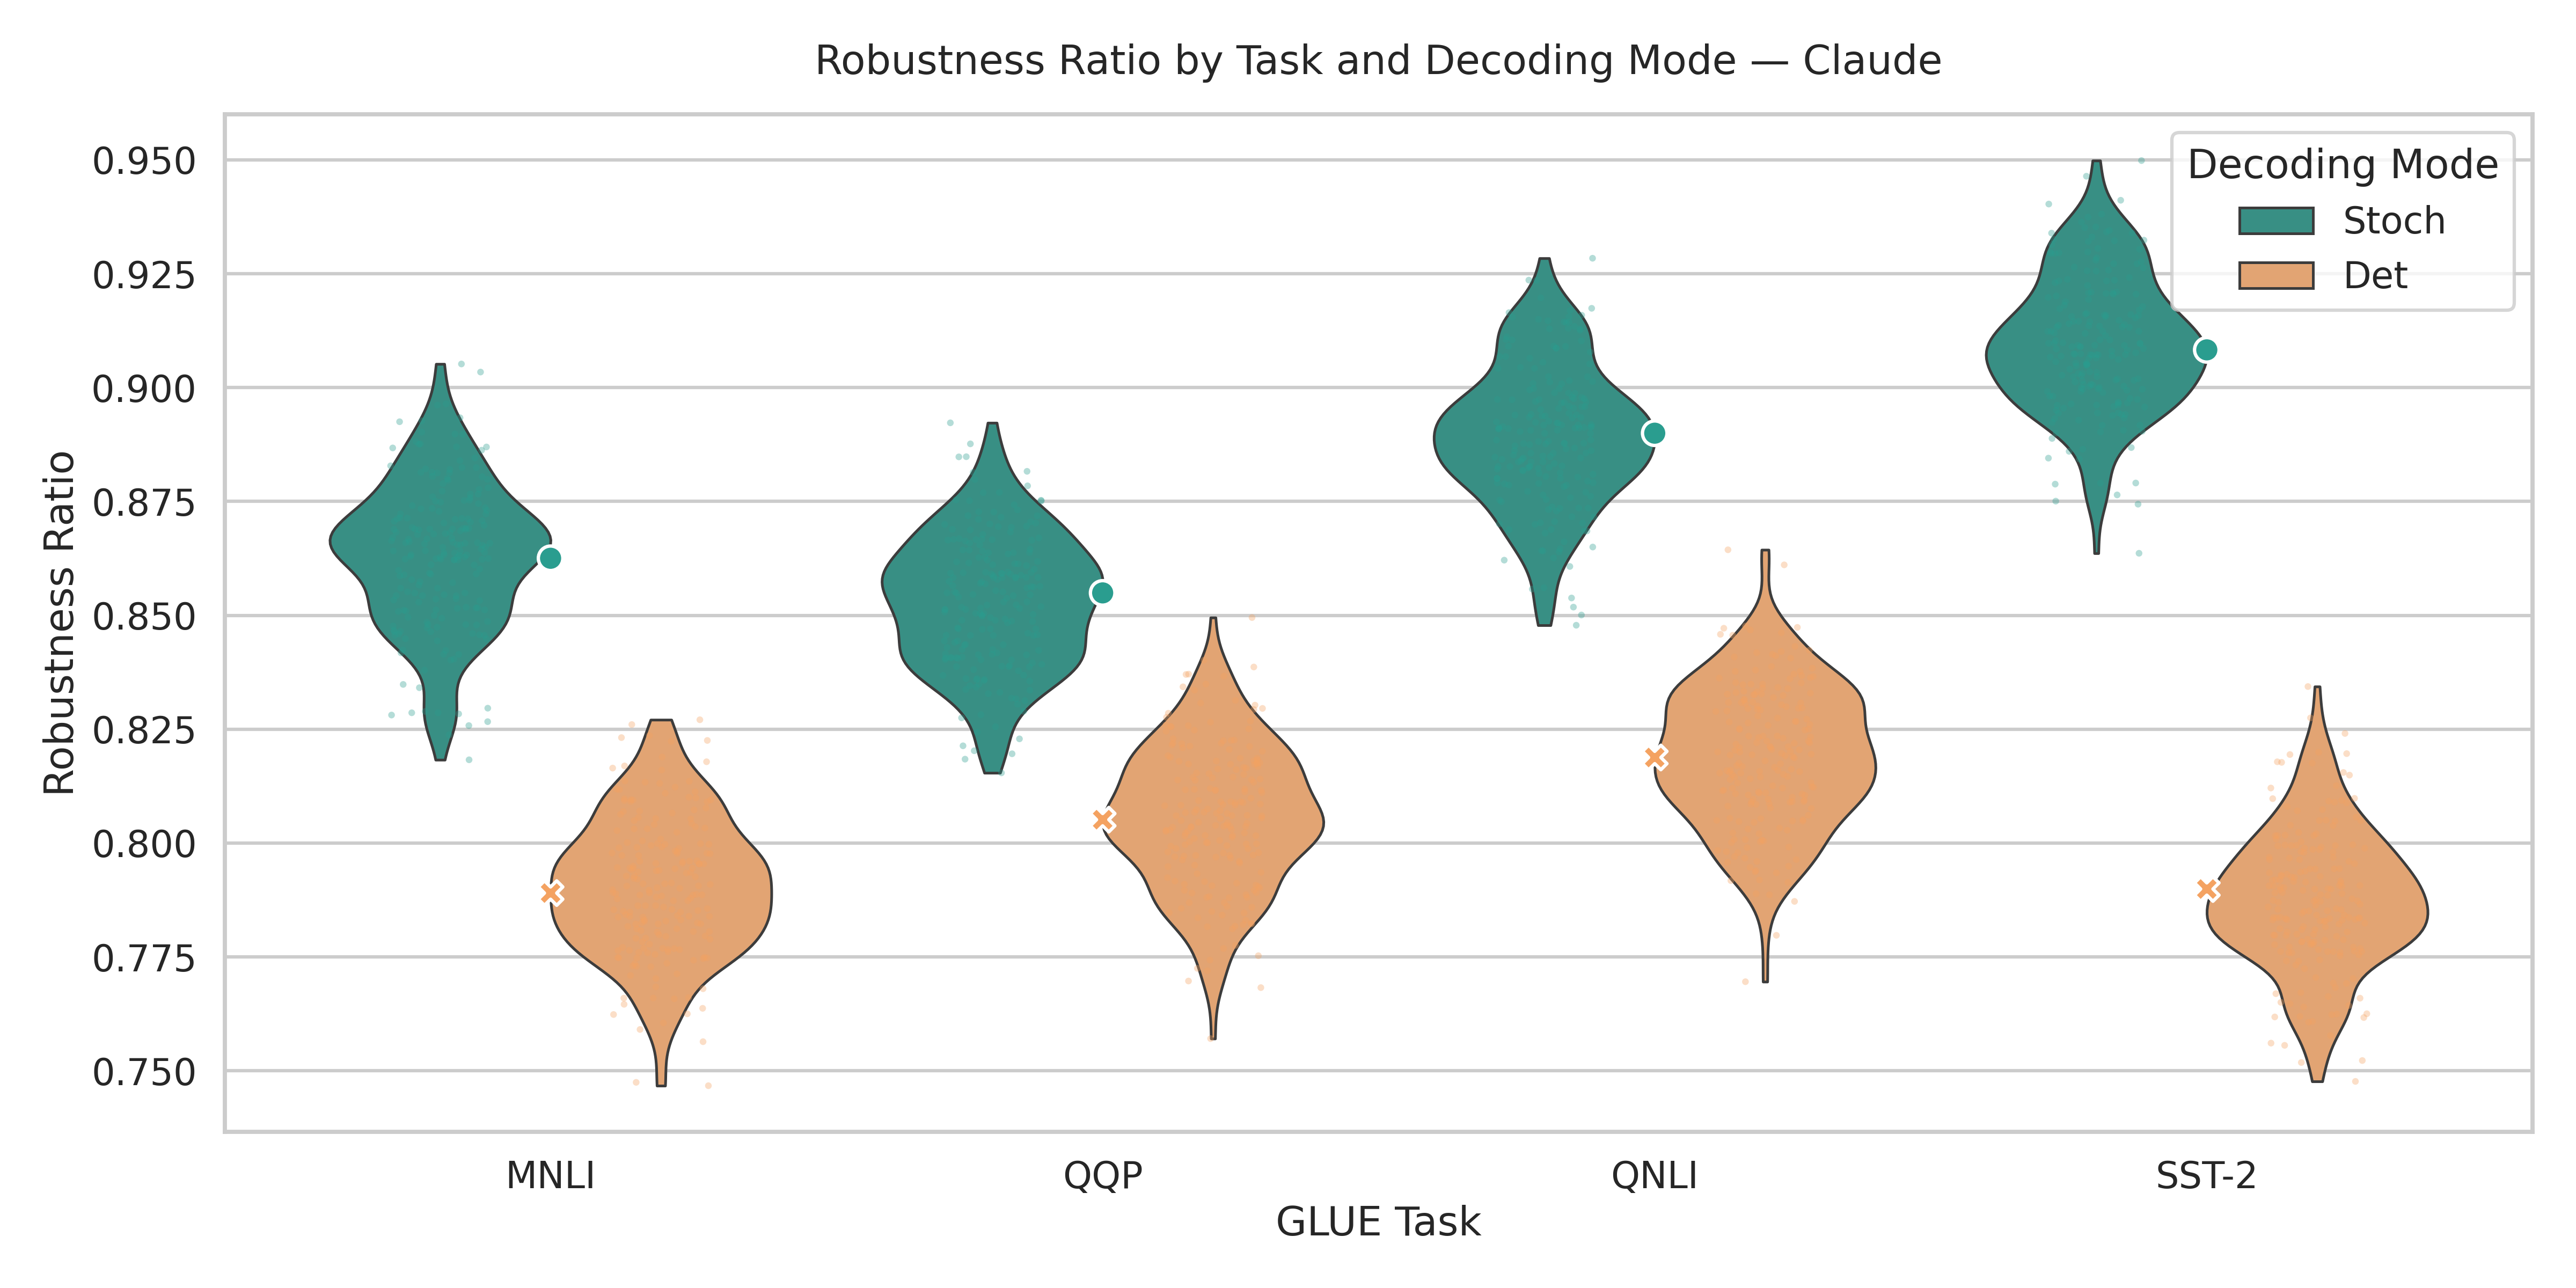
\includegraphics[width=\textwidth]{robustness_ratio/robustness_ratio_Claude.png}
  \caption{
  \textbf{Robustness ratios for \emph{Claude} across GLUE tasks.}
  Under \textbf{stochastic} decoding (teal), Claude attains robustness ratios between \(\mathbf{0.85}\) and \(\mathbf{0.91}\) across MNLI, QQP, QNLI, and SST-2, whereas \textbf{deterministic} decoding (orange) stays in the lower \(\mathbf{0.79\text{--}0.82}\) band.
  This yields absolute stochastic–deterministic gaps in the range of \(\mathbf{0.05\text{--}0.12}\).
  The tight stochastic violins on QNLI and SST-2 indicate \textbf{low variance across perturbation types}, while the slightly wider shapes on MNLI and QQP reveal \textbf{task-dependent sensitivity}.
  Overall, \emph{\textbf{Claude is consistently more robust when decoded stochastically}}, and the gains are not marginal but numerically substantial.
  }
  \label{fig:robustness-claude}
\end{figure*}

\begin{figure*}[t]
  \centering
  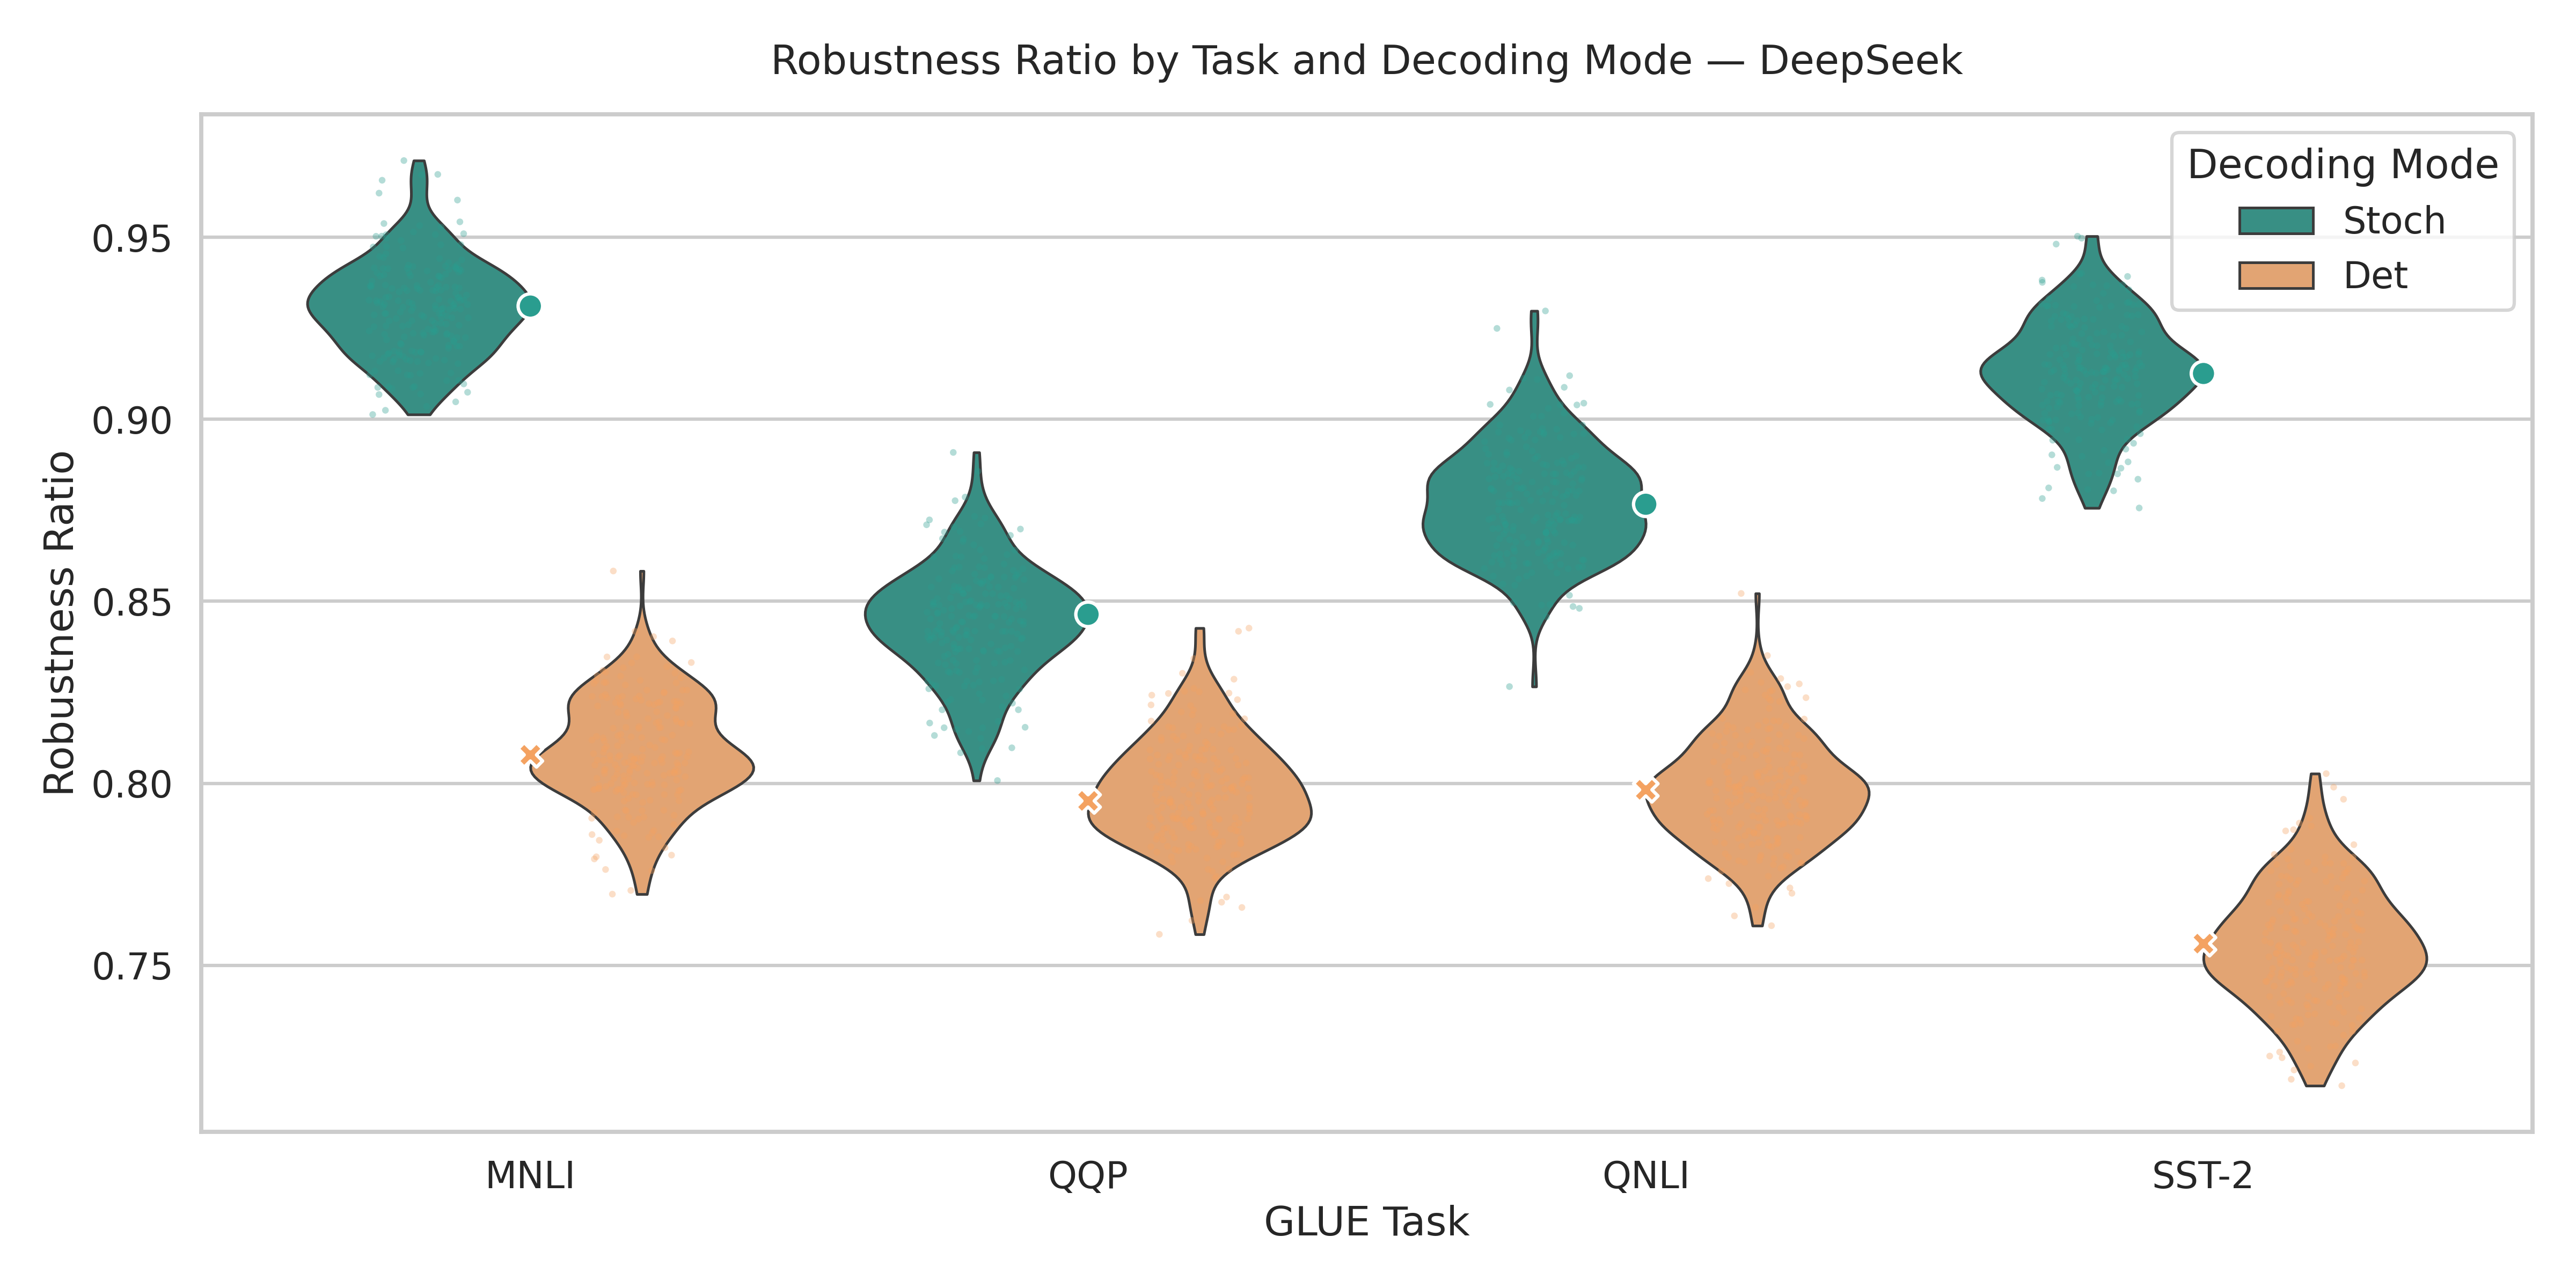
\includegraphics[width=\textwidth]{robustness_ratio/robustness_ratio_DeepSeek.png}
  \caption{
  \textbf{Robustness ratios for \emph{DeepSeek} across GLUE tasks.}
  \textbf{Stochastic decoding} places DeepSeek in a high-robustness regime, with ratios spanning \(\mathbf{0.85\text{--}0.93}\) across tasks, while \textbf{deterministic decoding} lags behind at \(\mathbf{0.76\text{--}0.81}\).
  The stochastic–deterministic gap ranges from about \(\mathbf{0.05}\) up to \(\mathbf{0.16}\) absolute points, making DeepSeek one of the models with the \textbf{largest decoding-induced robustness gains}.
  QNLI and SST-2 show the highest stochastic robustness, whereas MNLI and QQP display broader violins, reflecting \textbf{increased variability under perturbations}.
  These numbers highlight that \emph{\textbf{DeepSeek’s strong robustness is tightly coupled to stochastic inference}}; deterministic decoding leaves significant robustness “on the table.”
  }
  \label{fig:robustness-deepseek}
\end{figure*}

\begin{figure*}[t]
  \centering
  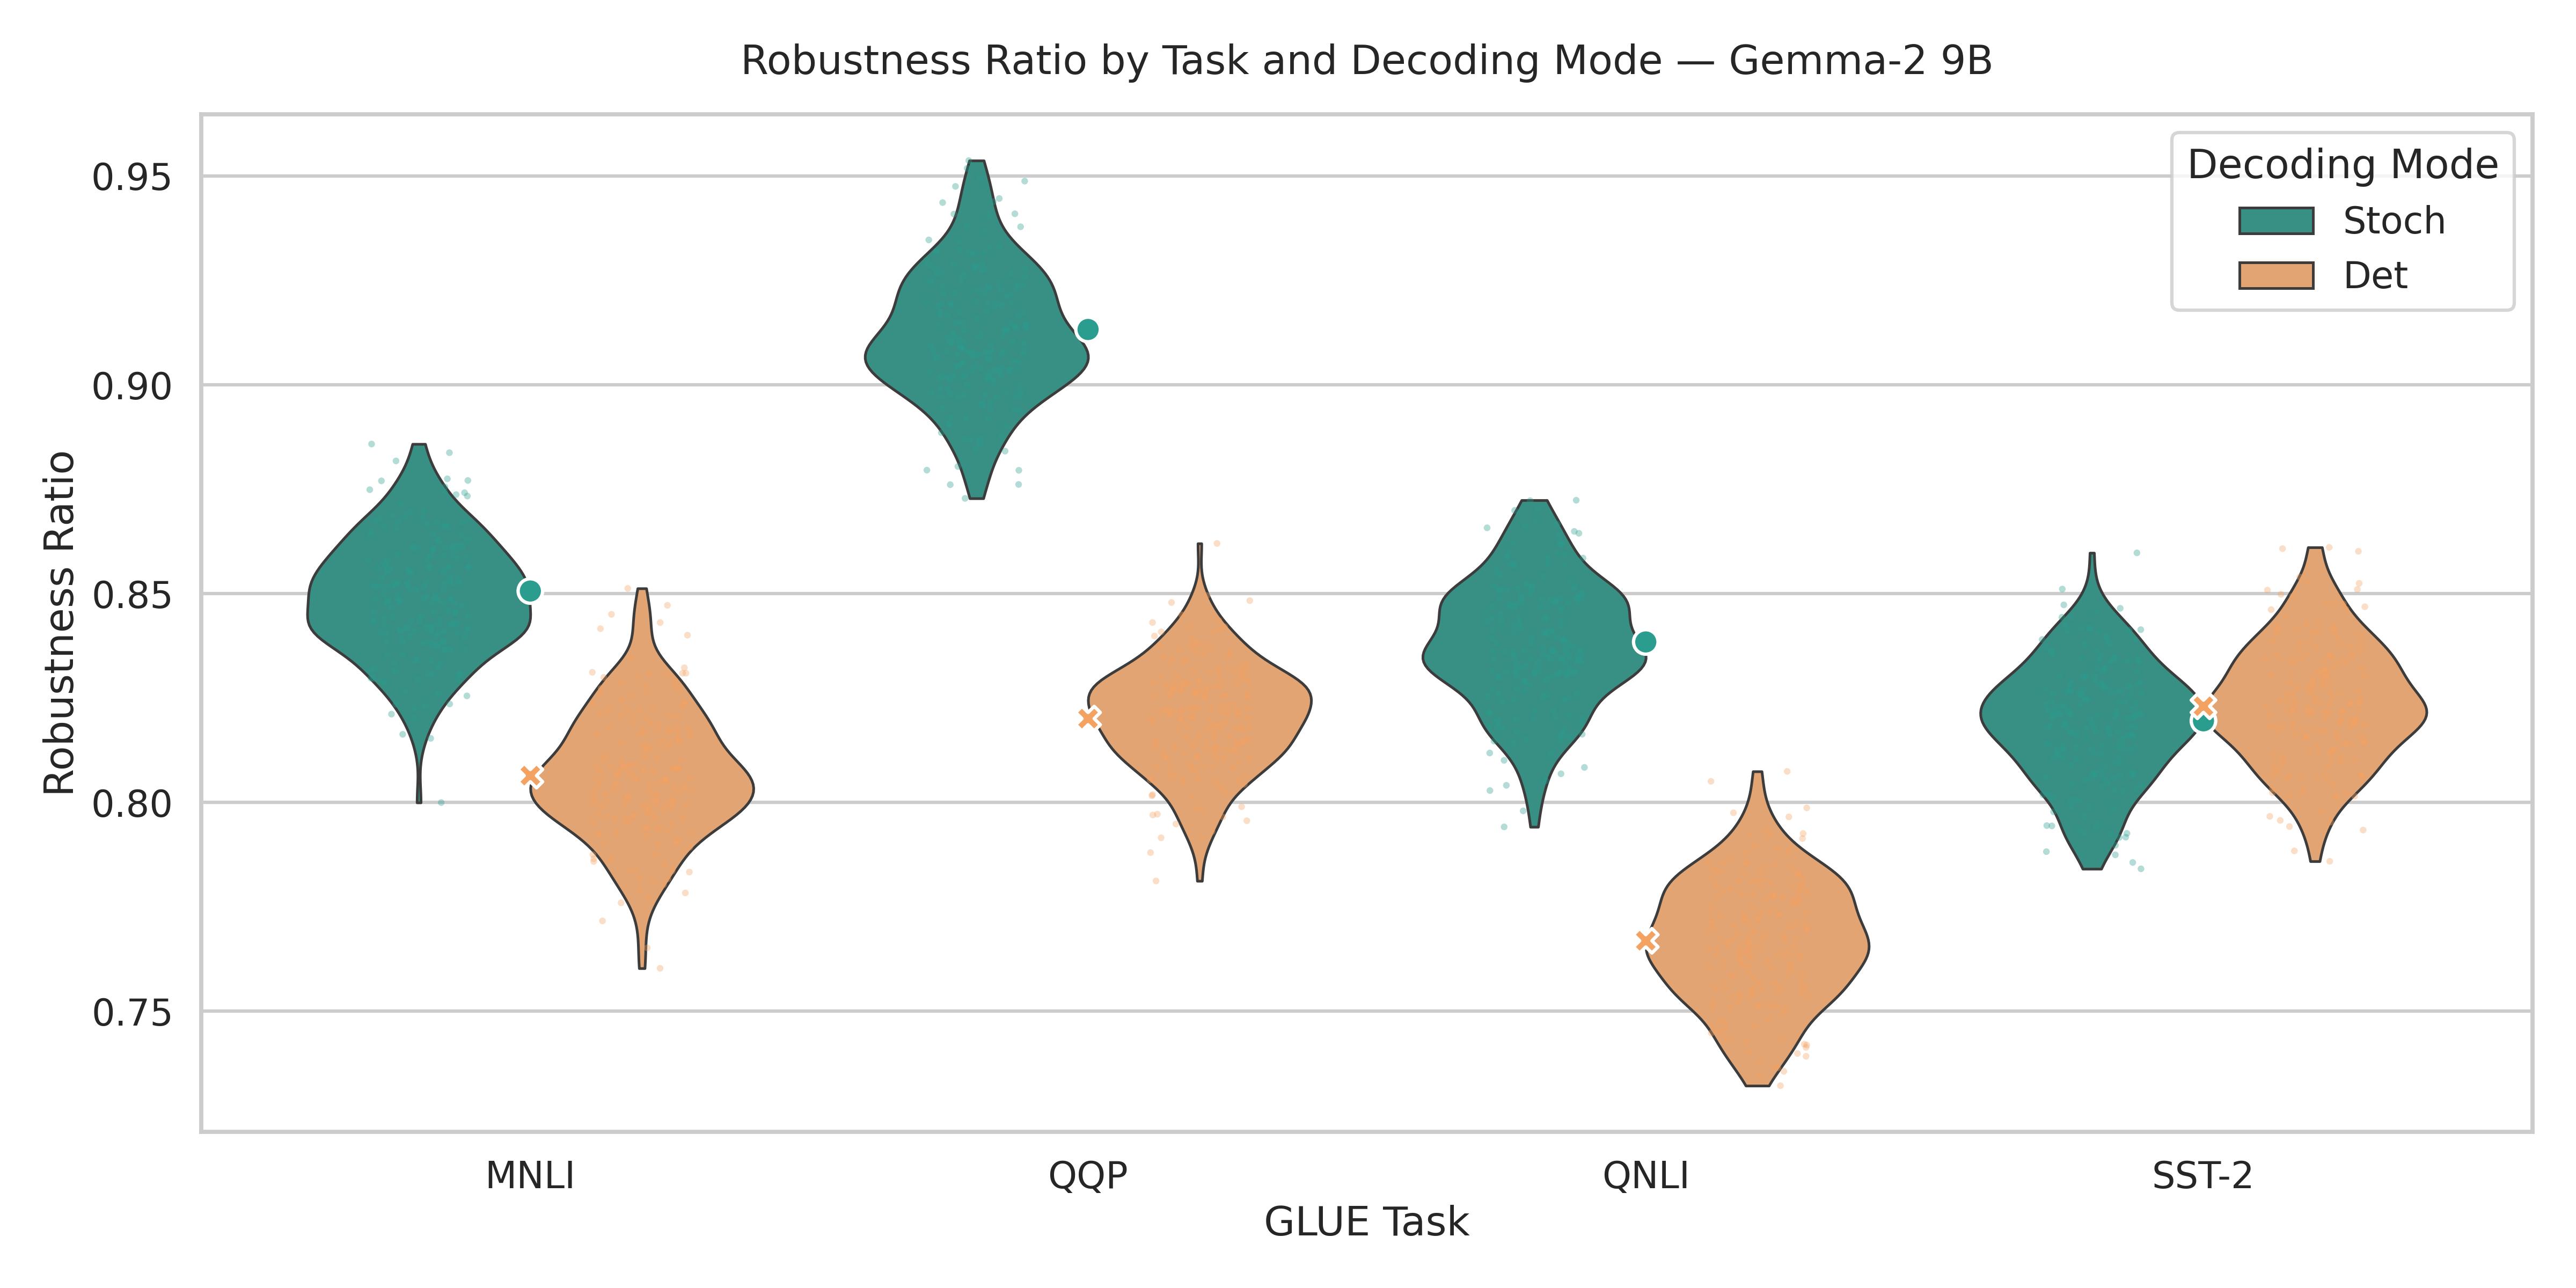
\includegraphics[width=\textwidth]{robustness_ratio/robustness_ratio_Gemma-2_9B.png}
  \caption{
  \textbf{Robustness ratios for \emph{Gemma-2 9B} across GLUE tasks.}
  With \textbf{stochastic} decoding, Gemma-2 9B achieves robustness ratios between \(\mathbf{0.82}\) and \(\mathbf{0.91}\), while \textbf{deterministic} decoding stays in the \(\mathbf{0.77\text{--}0.82}\) range.
  The task-wise stochastic–deterministic differences vary from essentially \(\mathbf{0.00}\) (one task where deterministic is on par) up to about \(\mathbf{0.09}\) absolute points.
  QQP and SST-2 show the \textbf{highest stochastic robustness}, while MNLI and QNLI are slightly lower and more spread out.
  This figure indicates that \emph{\textbf{even a mid-sized open model like Gemma-2 9B benefits measurably from stochastic decoding}}, though the magnitude of gains is somewhat smaller and more task-dependent than for frontier proprietary models.
  }
  \label{fig:robustness-gemma2-9b}
\end{figure*}

\begin{figure*}[t]
  \centering
  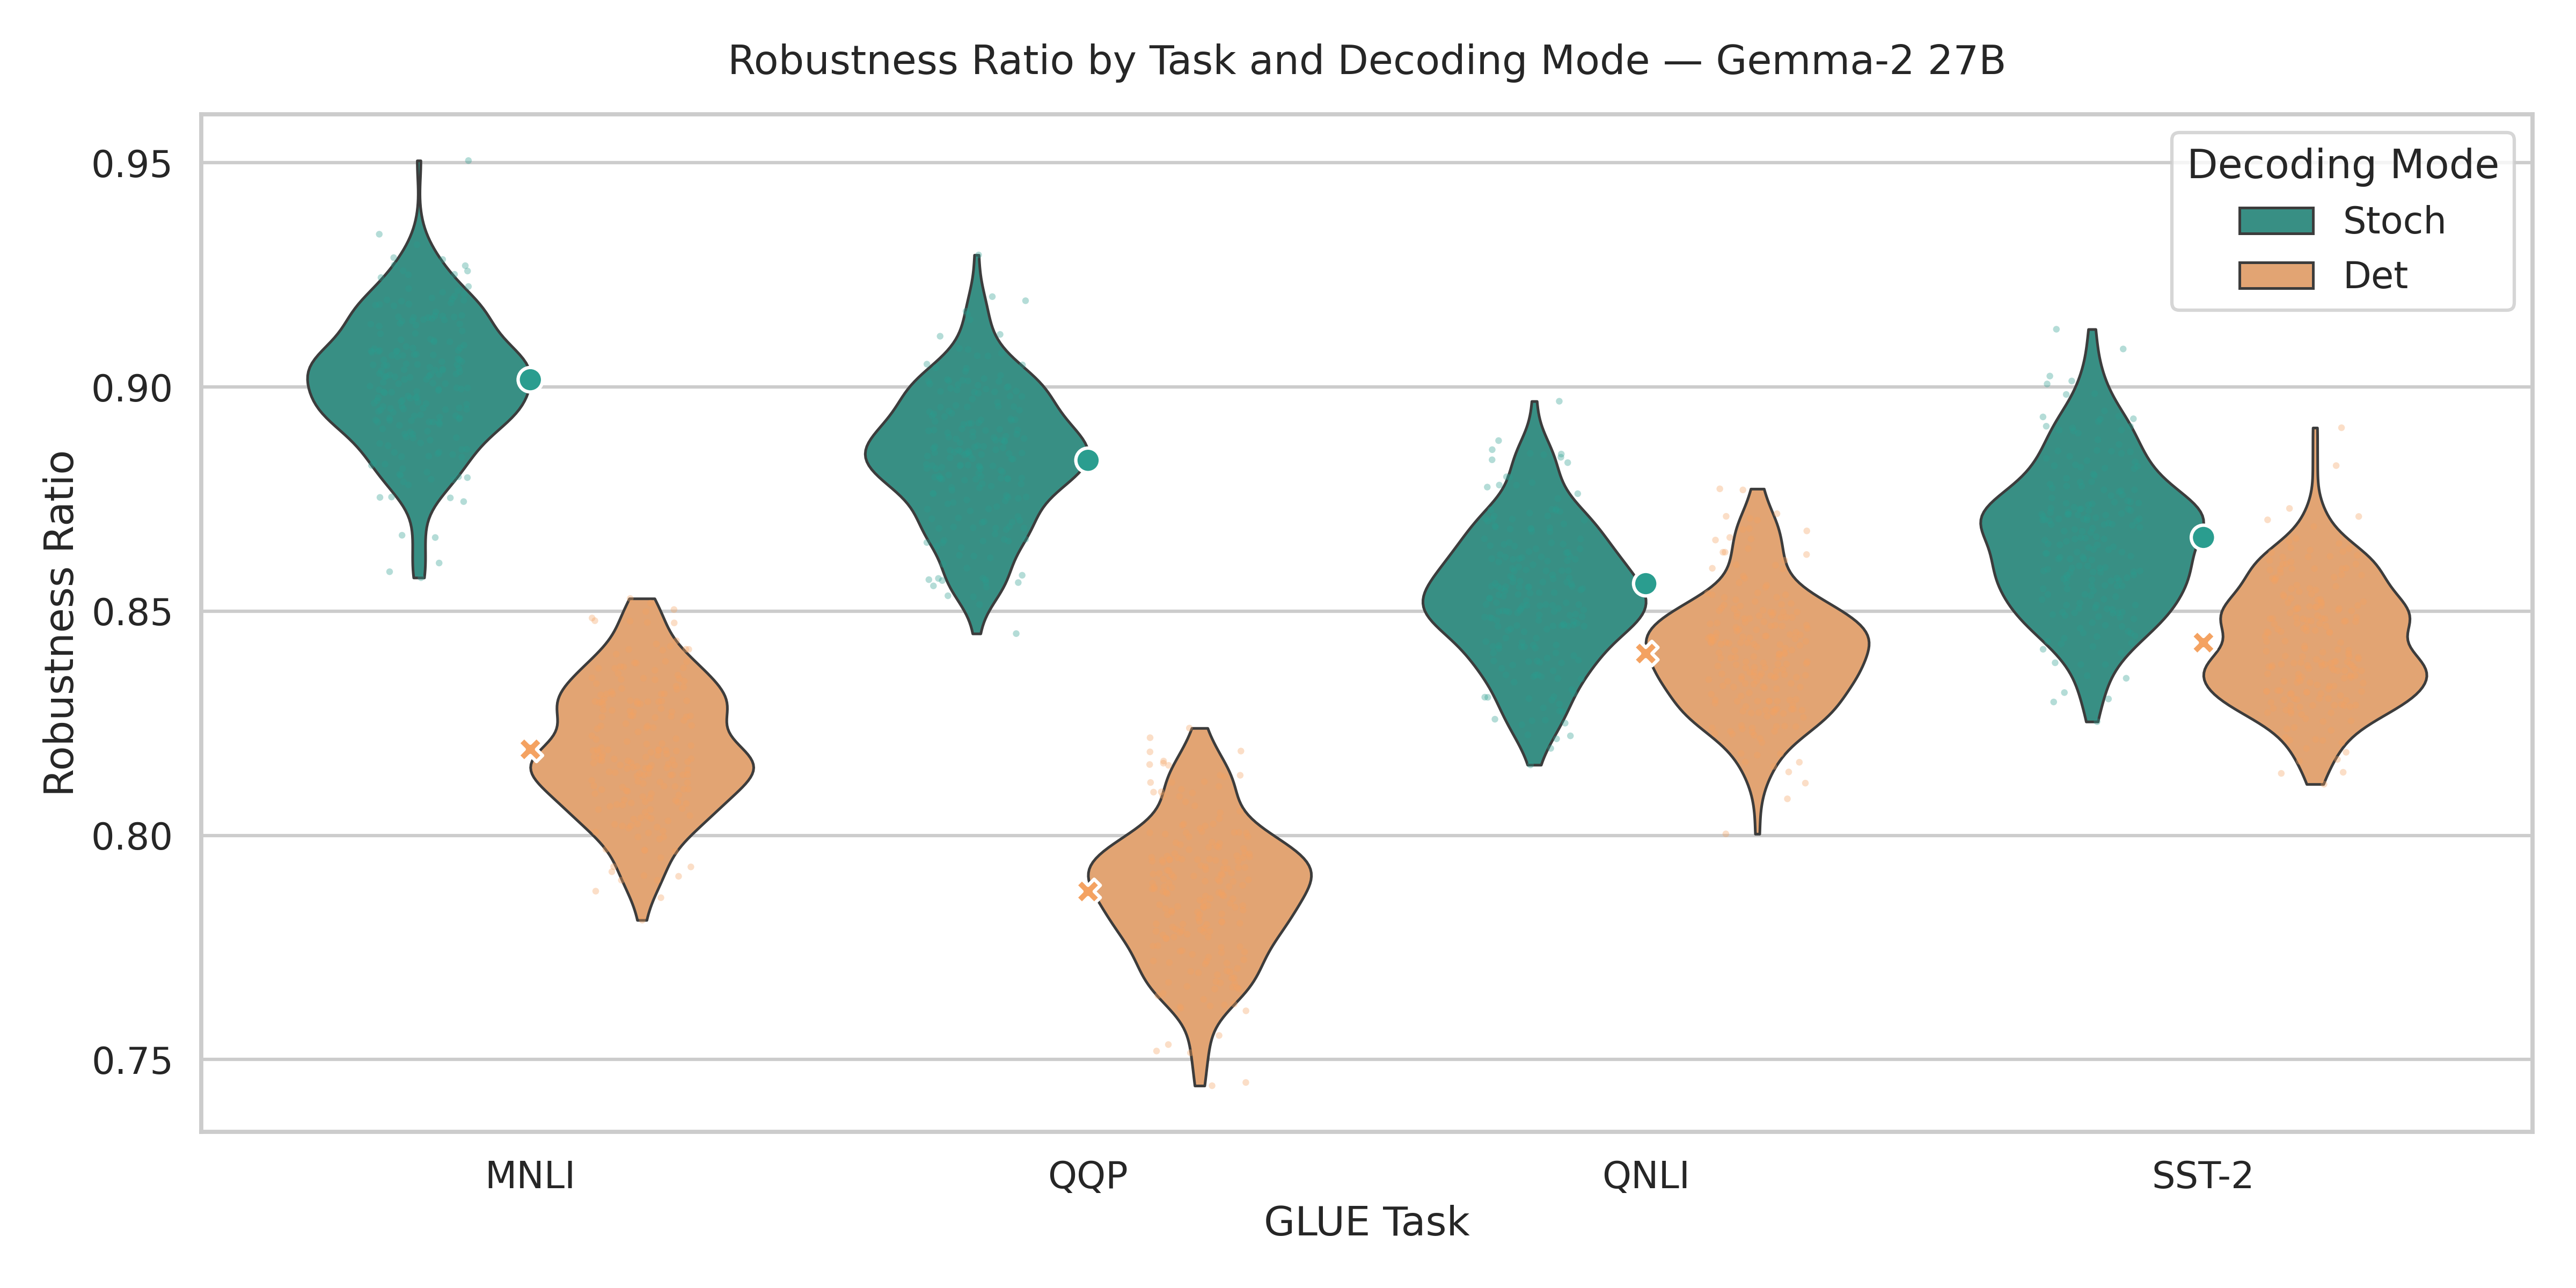
\includegraphics[width=\textwidth]{robustness_ratio/robustness_ratio_Gemma-2_27B.png}
  \caption{
  \textbf{Robustness ratios for \emph{Gemma-2 27B} across GLUE tasks.}
  Scaling to 27B pushes the \textbf{stochastic robustness} band to \(\mathbf{0.86\text{--}0.90}\), while \textbf{deterministic} decoding lies in the slightly lower interval \(\mathbf{0.79\text{--}0.84}\).
  Stochastic–deterministic gaps span roughly \(\mathbf{0.02\text{--}0.10}\) across tasks, smaller than for some proprietary models but still \textbf{systematically positive}.
  MNLI and QQP show clear upward shifts compared to Gemma-2 9B, and SST-2 reaches the top of the model’s robustness range with \textbf{narrow, high violins}.
  The combination of higher means and reduced spread suggests that \emph{\textbf{Gemma-2 27B is both more robust and more stable}}, yet still meaningfully boosted by stochastic decoding.
  }
  \label{fig:robustness-gemma2-27b}
\end{figure*}

\begin{figure*}[t]
  \centering
  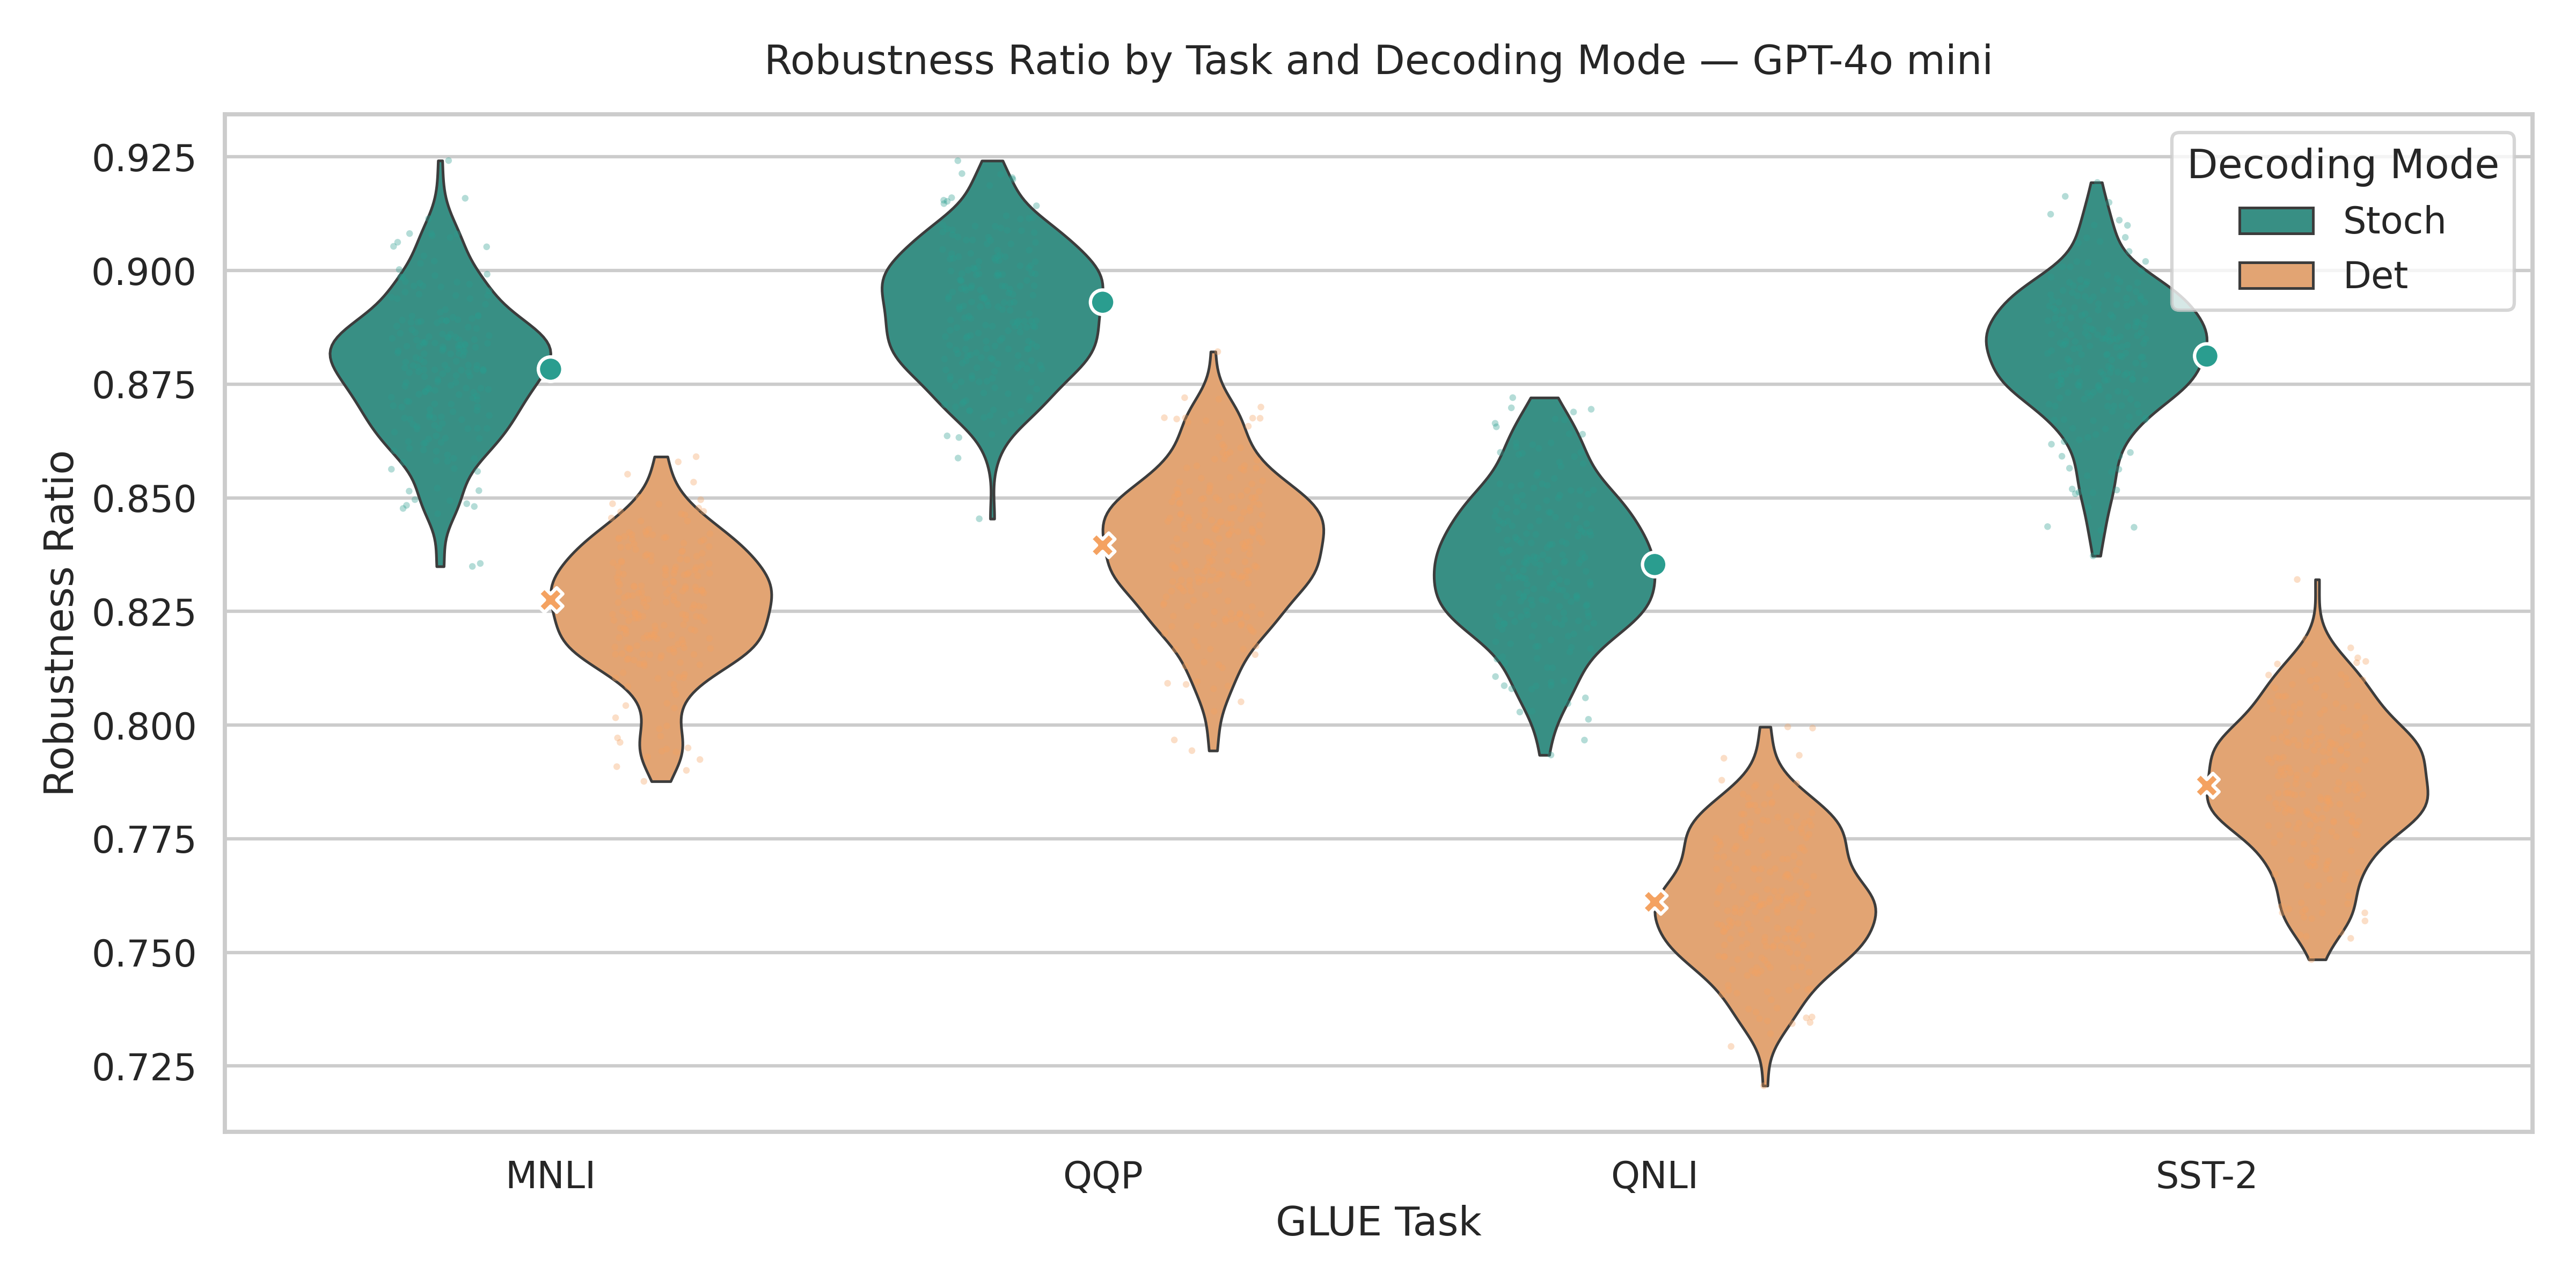
\includegraphics[width=\textwidth]{robustness_ratio/robustness_ratio_GPT-4o_mini.png}
  \caption{
  \textbf{Robustness ratios for \emph{GPT-4o mini} across GLUE tasks.}
  Under \textbf{stochastic} decoding, GPT-4o mini attains robustness ratios in the \(\mathbf{0.84\text{--}0.89}\) range, whereas \textbf{deterministic} decoding falls between \(\mathbf{0.76}\) and \(\mathbf{0.84}\).
  The resulting gaps are on the order of \(\mathbf{0.05\text{--}0.09}\) absolute points depending on the task.
  MNLI and QQP sit around the lower end of the stochastic band, while QNLI and especially SST-2 approach the top, indicating that \textbf{classification-style tasks can remain robust even for a compressed model}.
  These numeric ranges show that \emph{\textbf{even a distilled GPT-4o variant retains a sizable robustness margin under stochastic decoding}}, making inference-time choices crucial when deploying lightweight models.
  }
  \label{fig:robustness-gpt4o-mini}
\end{figure*}

\begin{figure*}[t]
  \centering
  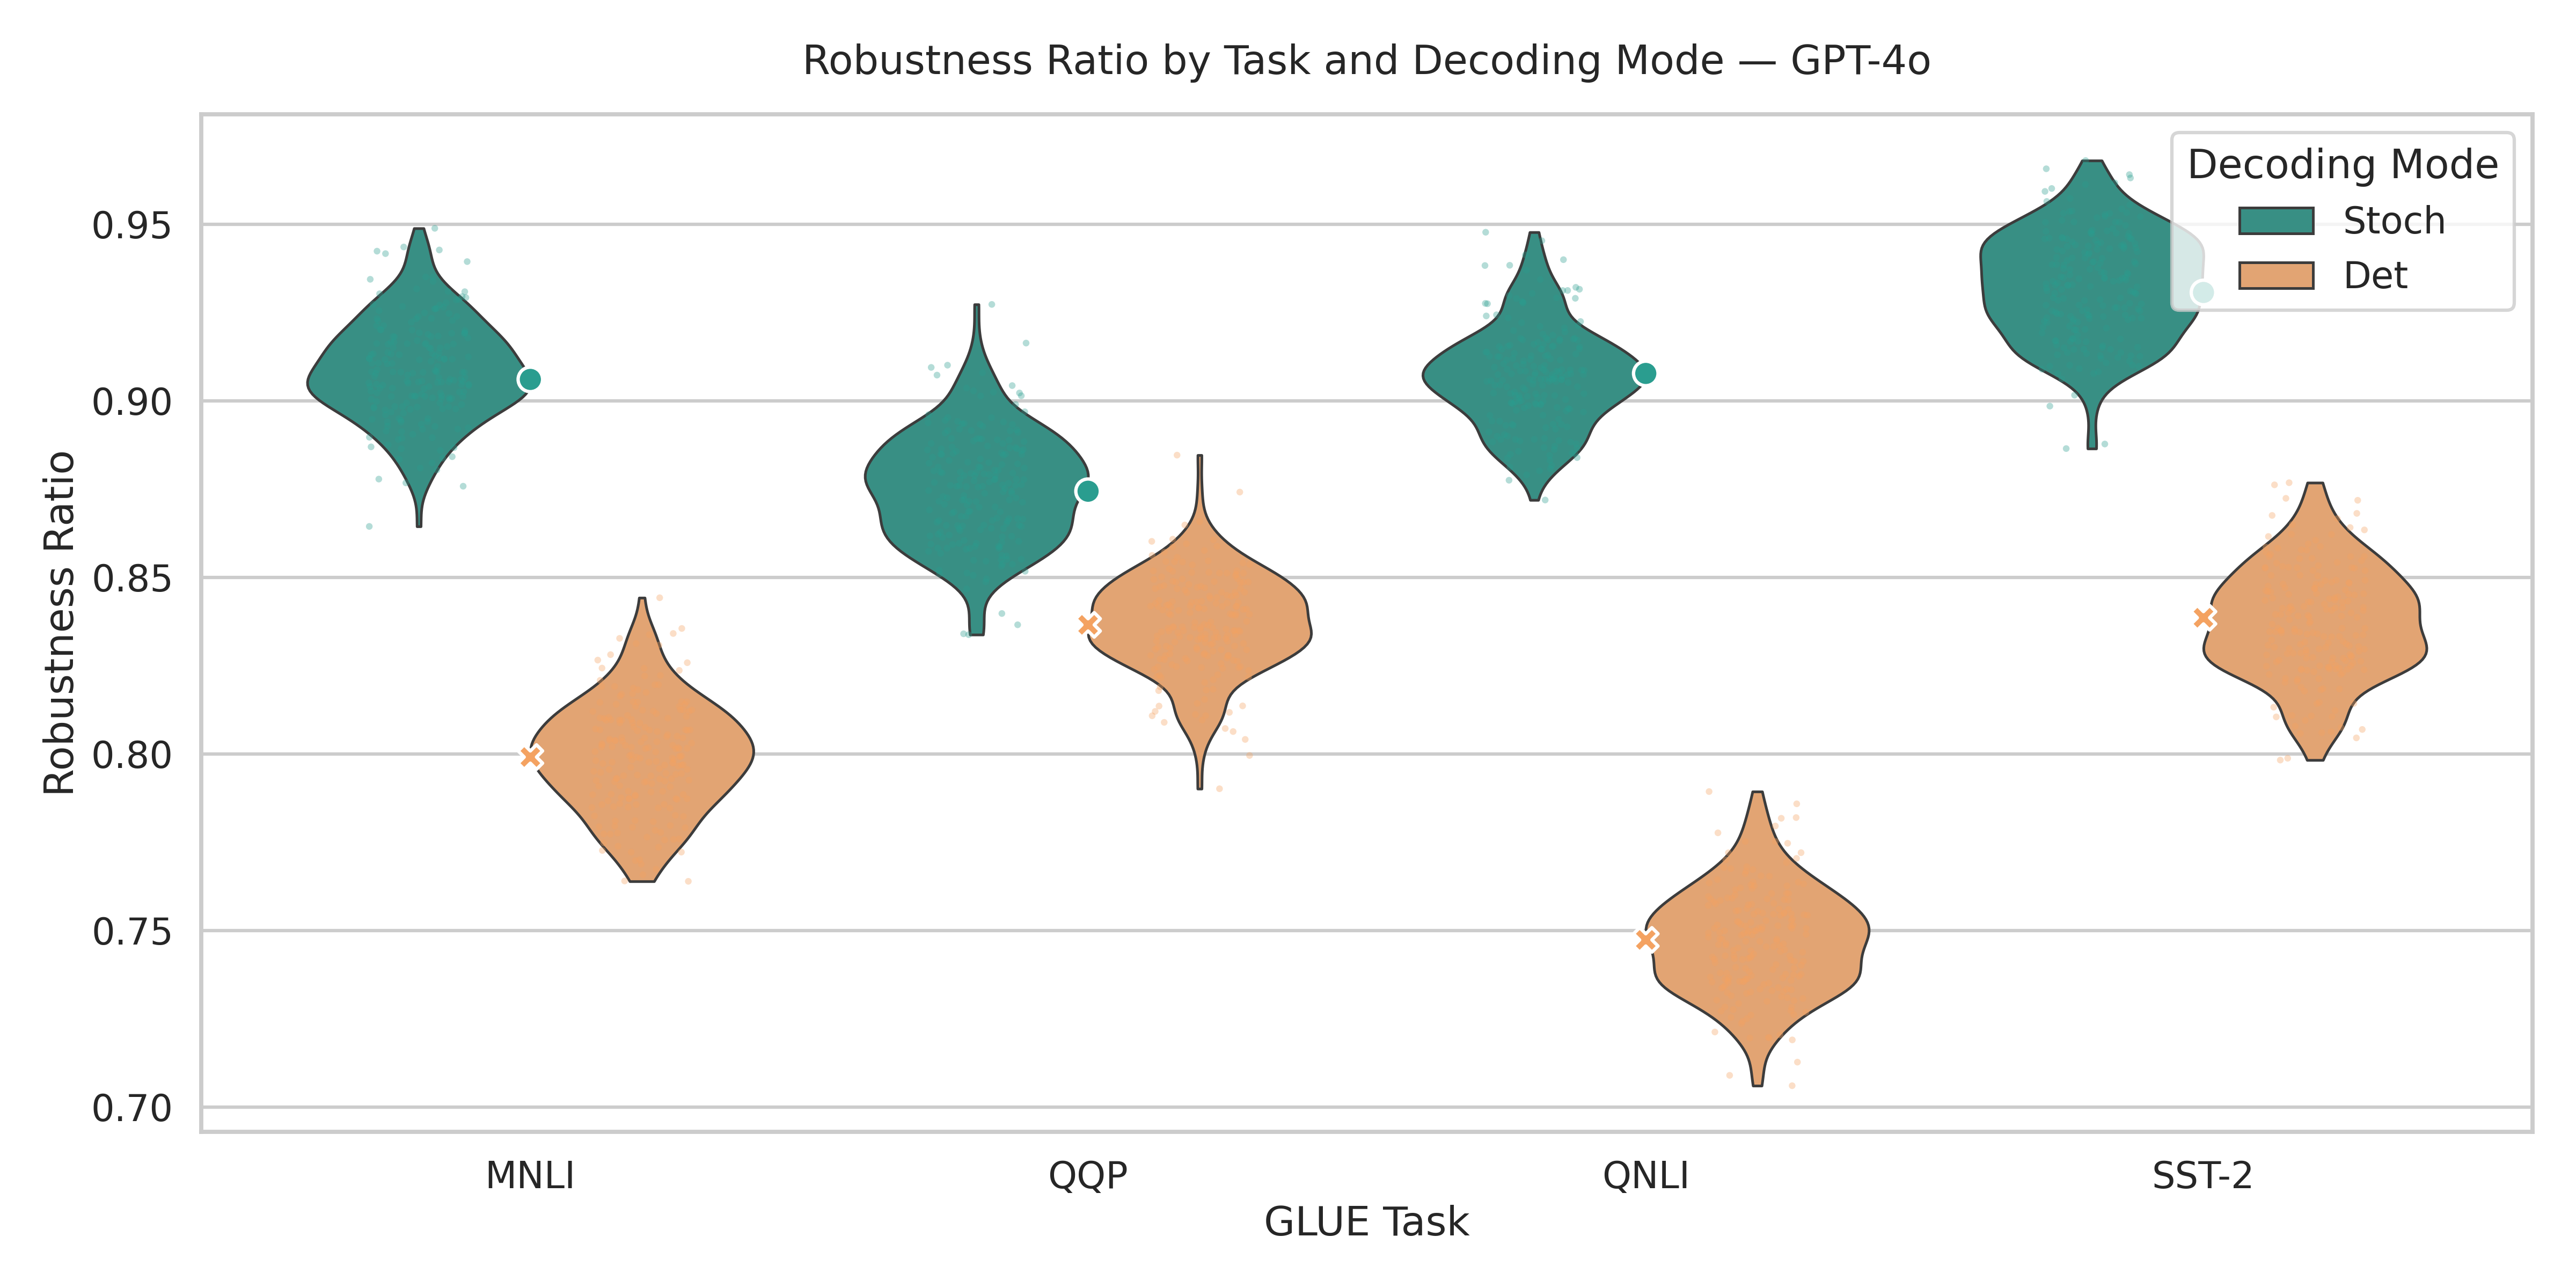
\includegraphics[width=\textwidth]{robustness_ratio/robustness_ratio_GPT-4o.png}
  \caption{
  \textbf{Robustness ratios for \emph{GPT-4o} across GLUE tasks.}
  GPT-4o shows one of the \textbf{strongest robustness profiles}: stochastic ratios consistently lie between \(\mathbf{0.87}\) and \(\mathbf{0.93}\), while deterministic decoding drops to \(\mathbf{0.75\text{--}0.84}\).
  Task-wise stochastic–deterministic gaps range from about \(\mathbf{0.04}\) up to \(\mathbf{0.16}\) absolute points, with the largest differences on QNLI and SST-2.
  The tight, high violins for stochastic decoding indicate \textbf{high robustness and low variance}, whereas deterministic violins are wider and noticeably shifted down.
  These results underscore that \emph{\textbf{GPT-4o’s robustness is not merely a property of the underlying model but also of the decoding policy}}: deterministic inference underutilizes its potential.
  }
  \label{fig:robustness-gpt4o}
\end{figure*}

\begin{figure*}[t]
  \centering
  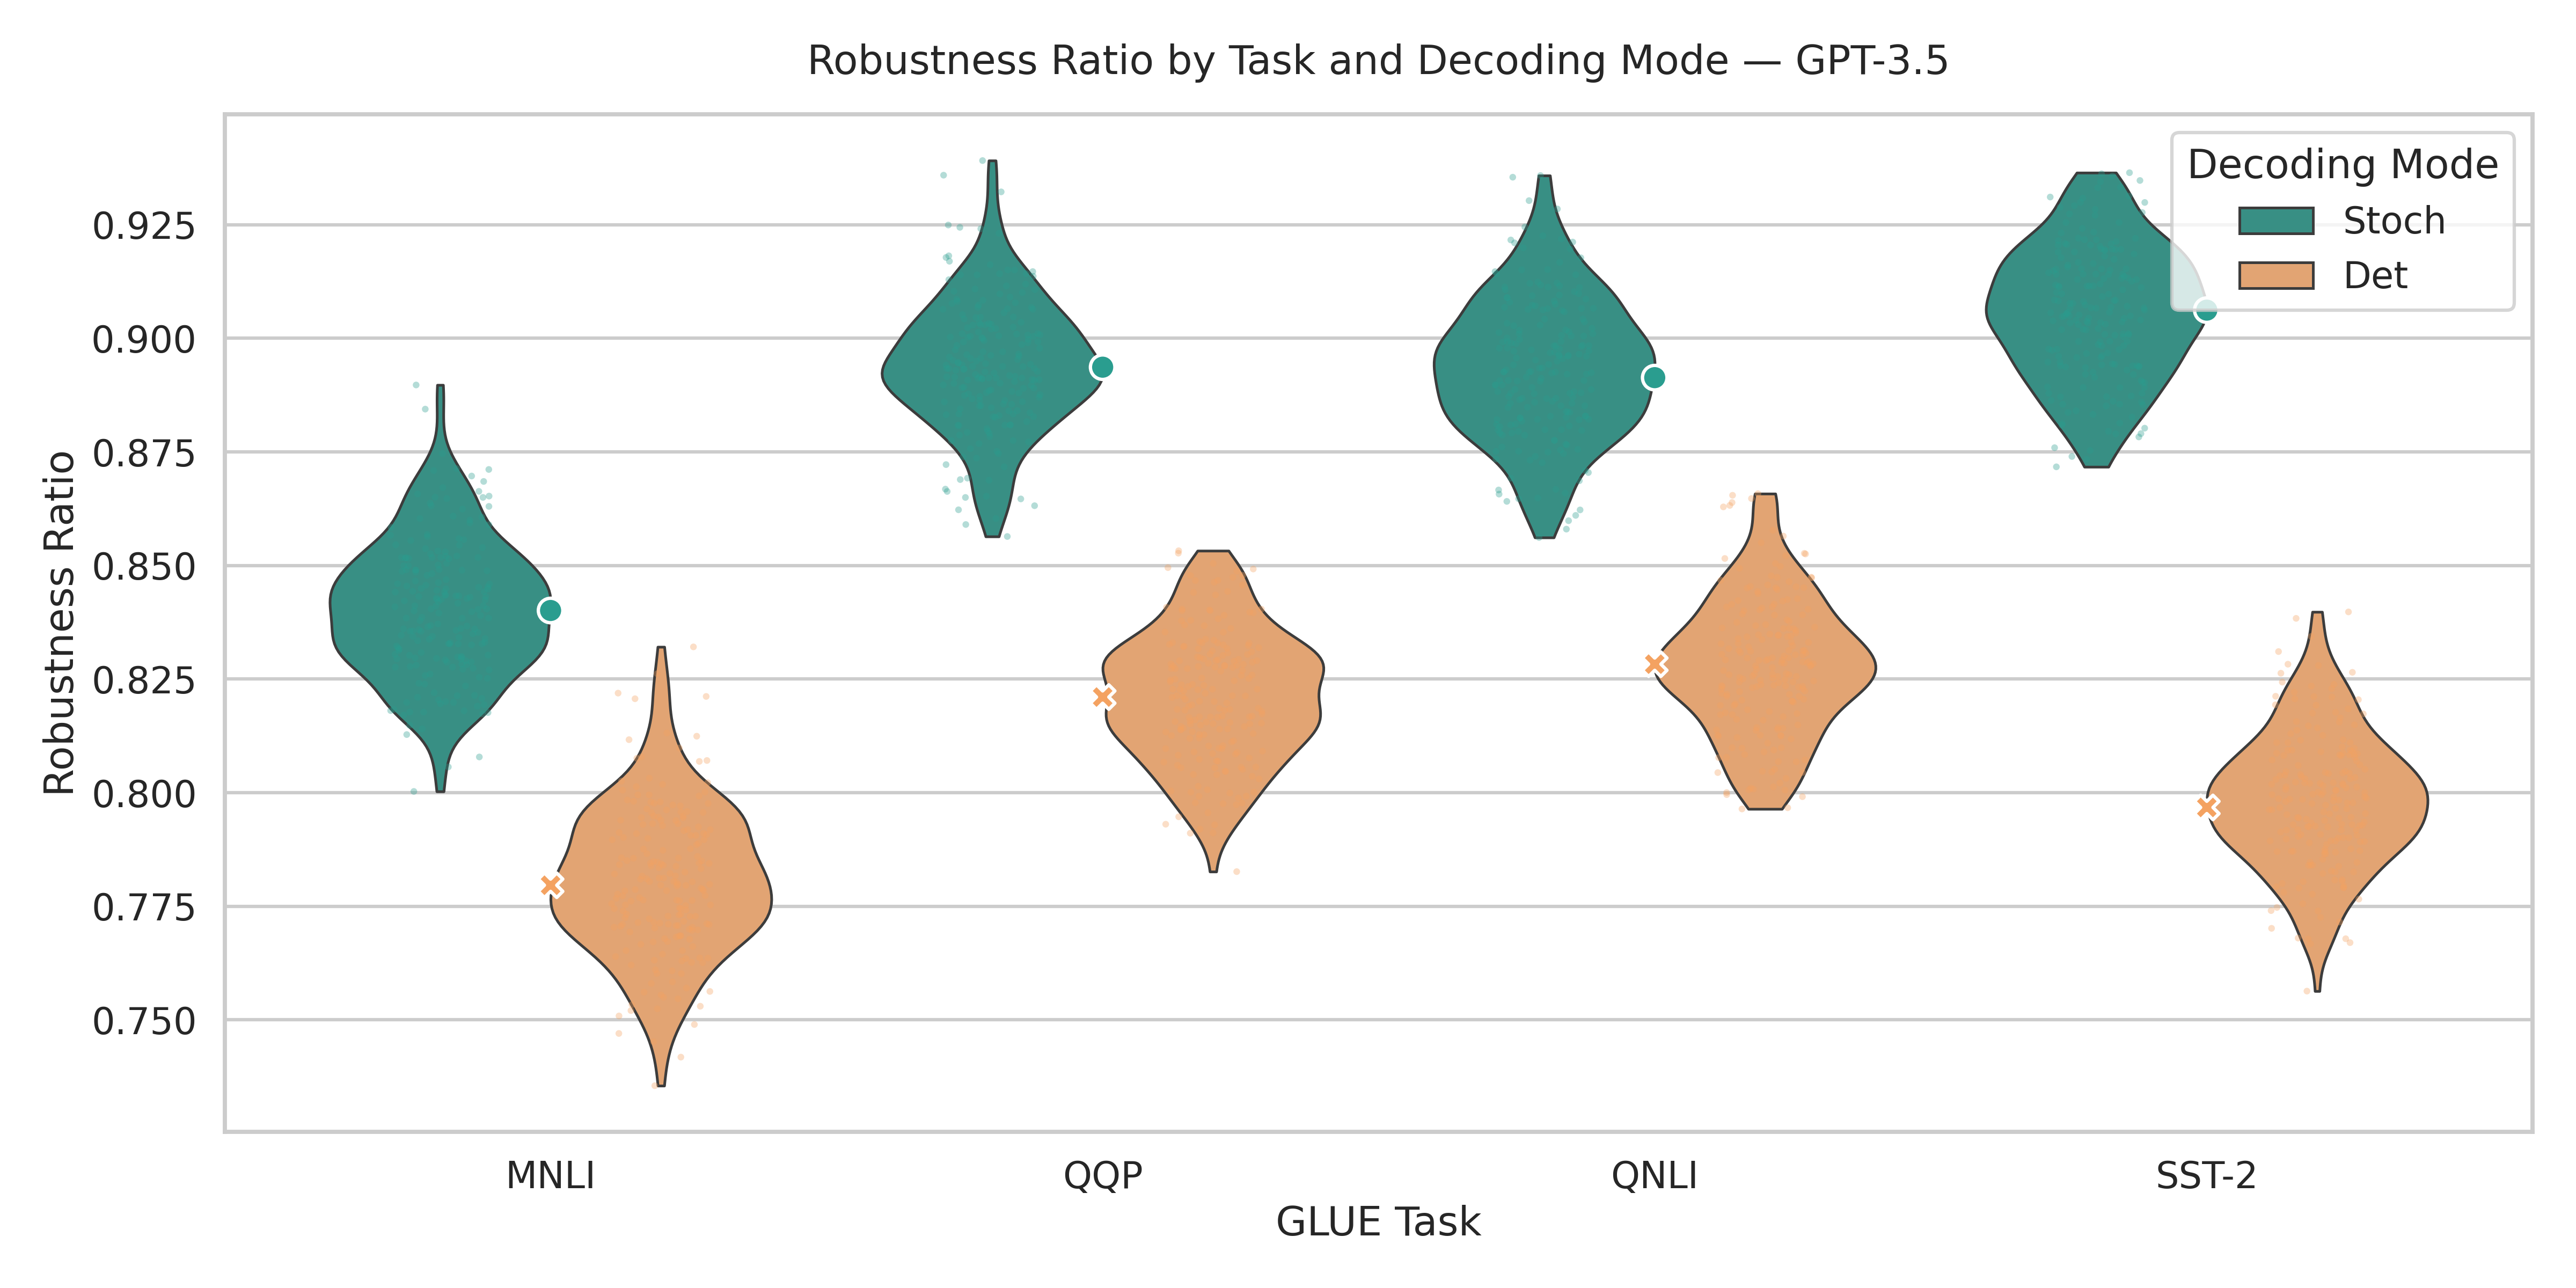
\includegraphics[width=\textwidth]{robustness_ratio/robustness_ratio_GPT-35.png}
  \caption{
  \textbf{Robustness ratios for \emph{GPT-3.5} across GLUE tasks.}
  For \textbf{stochastic} decoding, robustness ratios span \(\mathbf{0.84\text{--}0.91}\), situating GPT-3.5 below GPT-4o but still in a relatively strong band.
  \textbf{Deterministic} decoding compresses the model into the \(\mathbf{0.78\text{--}0.83}\) range, with per-task gaps of roughly \(\mathbf{0.06\text{--}0.11}\) absolute points.
  QQP and MNLI exhibit the \textbf{largest downward shifts and broader violins} under deterministic decoding, signaling heightened vulnerability to adversarial paraphrases in these settings.
  Taken together, the figure positions \emph{\textbf{GPT-3.5 as a mid-robustness baseline whose observed robustness is highly sensitive to decoding}}: small sampling changes can translate into \(\mathbf{5\text{--}10}\,\)pp differences in robustness ratio.
  }
  \label{fig:robustness-gpt35}
\end{figure*}

\begin{figure*}[t]
  \centering
  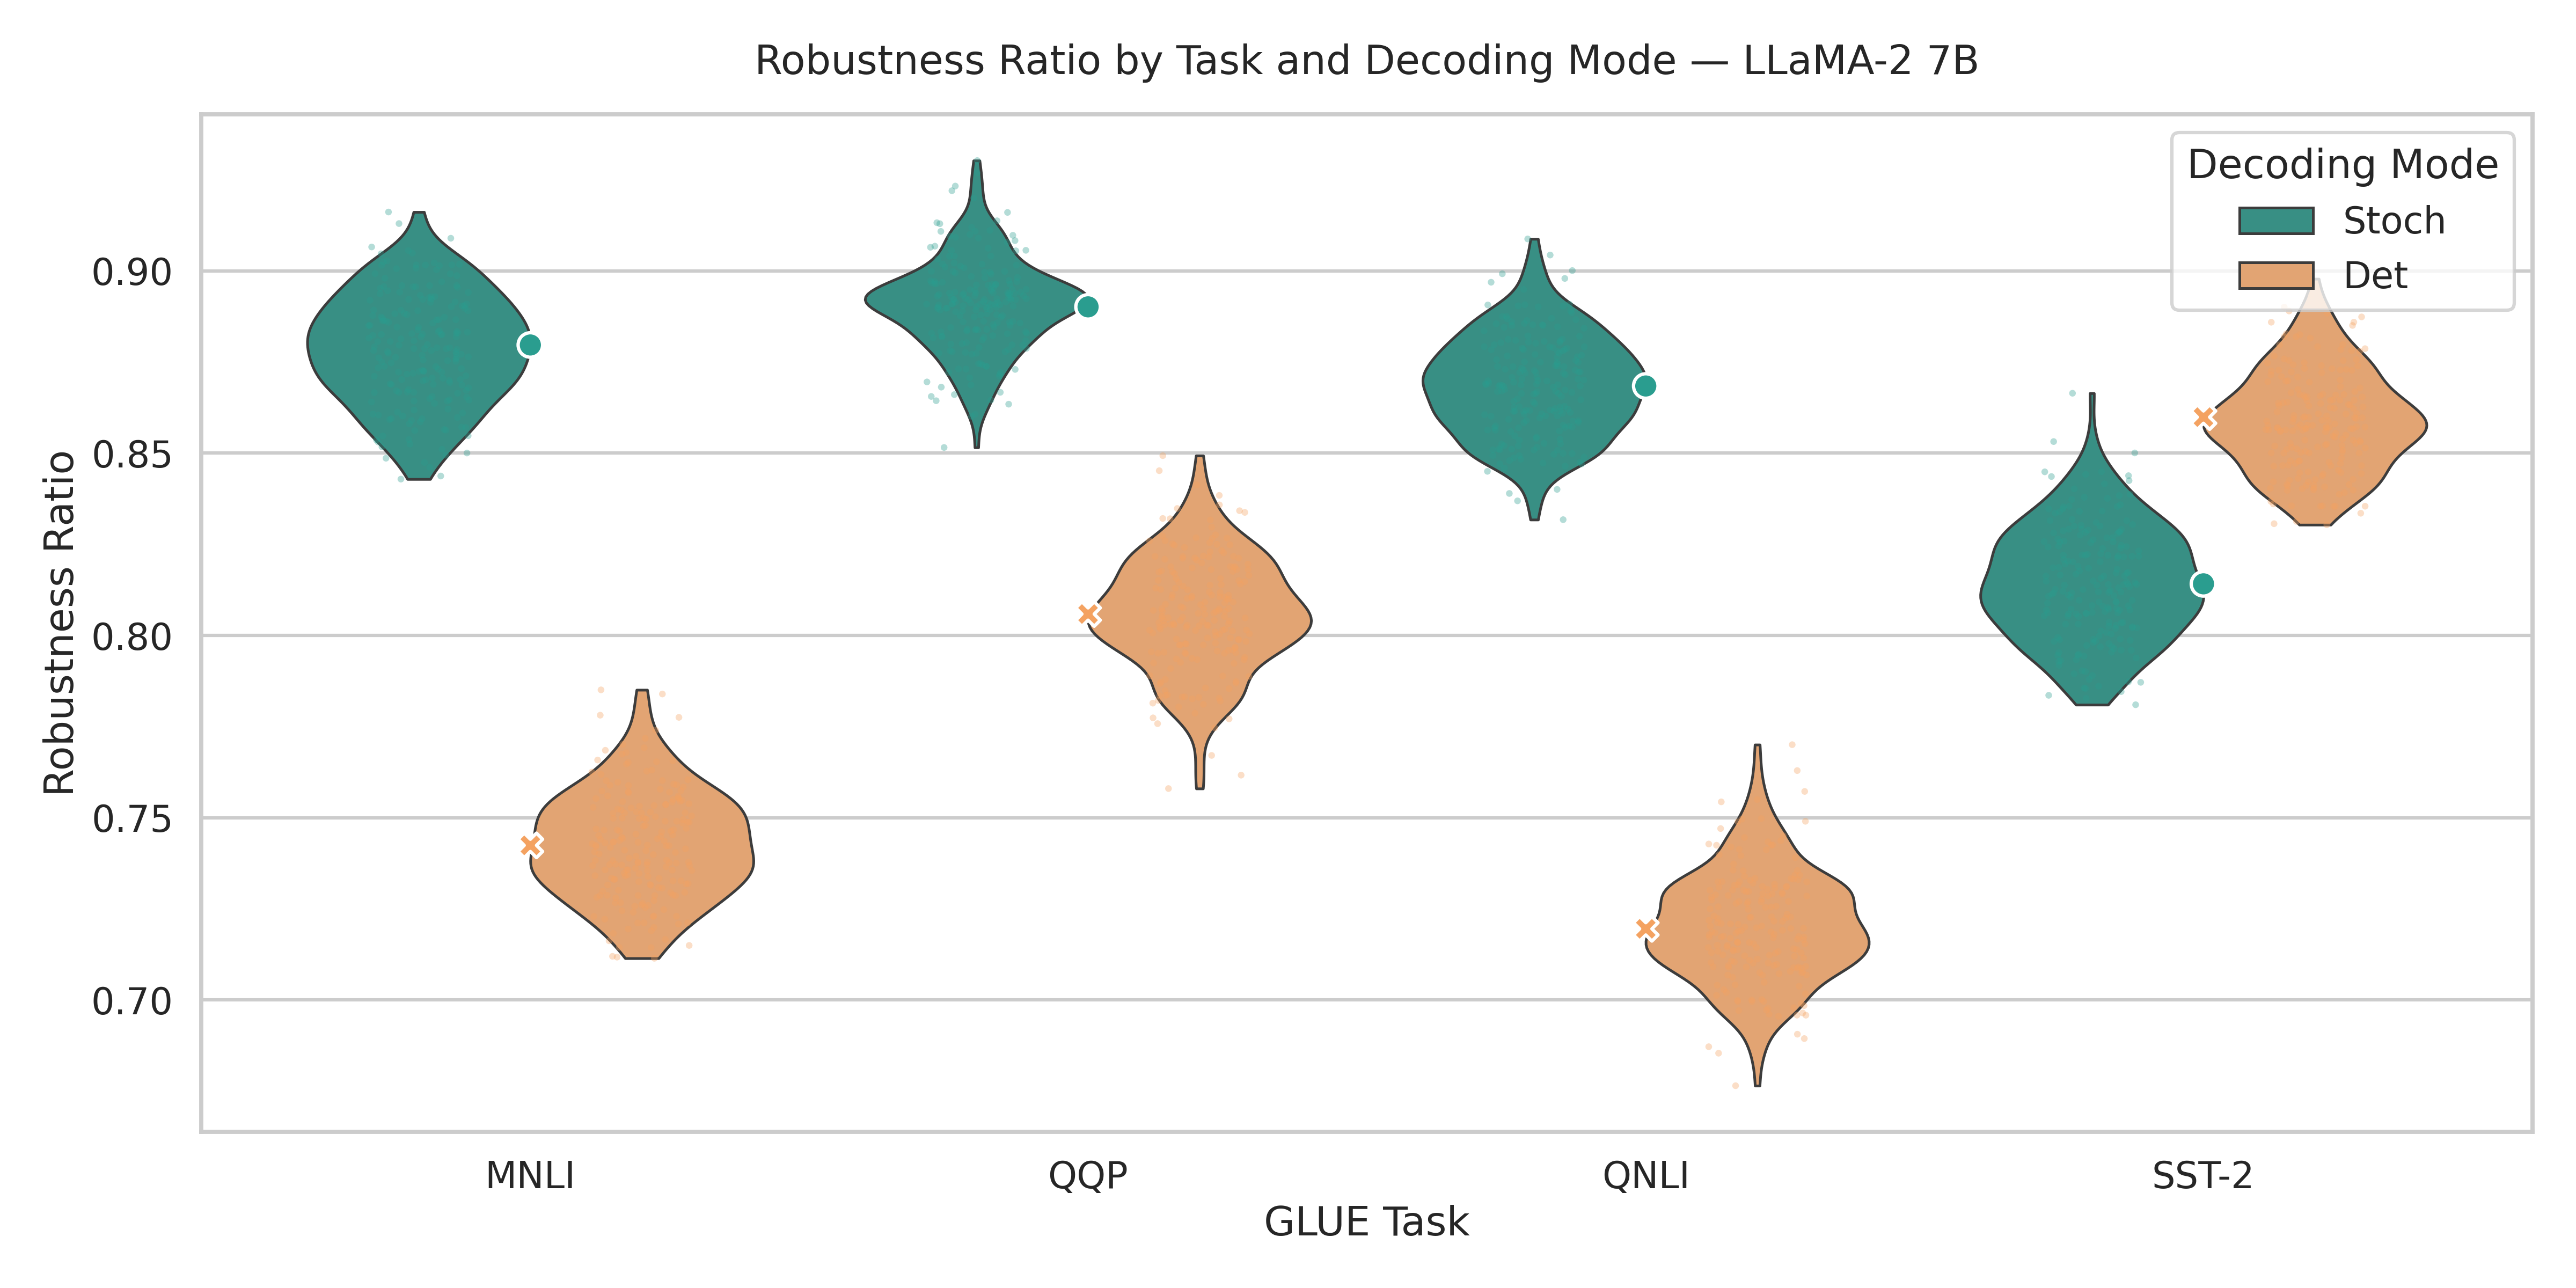
\includegraphics[width=\textwidth]{robustness_ratio/robustness_ratio_LLaMA-2_7B.png}
  \caption{
  \textbf{Robustness ratios for \emph{LLaMA-2 7B} across GLUE tasks.}
  \textbf{Stochastic} decoding yields robustness ratios between \(\mathbf{0.81}\) and \(\mathbf{0.89}\), while \textbf{deterministic} decoding ranges more widely from \(\mathbf{0.72}\) up to \(\mathbf{0.86}\).
  The stochastic–deterministic differences vary from a slight negative value (one task where deterministic happens to be slightly higher) to a substantial positive gap of about \(\mathbf{0.15}\) absolute points.
  MNLI and QNLI show the \textbf{lowest medians and widest violins}, indicating that a 7B-class open model struggles most on inference-style tasks under perturbations.
  Numerically, this figure illustrates that \emph{\textbf{LLaMA-2 7B sits at the lower end of the robustness spectrum and is highly decoding-sensitive}}, making it an informative but fragile baseline.
  }
  \label{fig:robustness-llama2-7b}
\end{figure*}

\begin{figure*}[t]
  \centering
  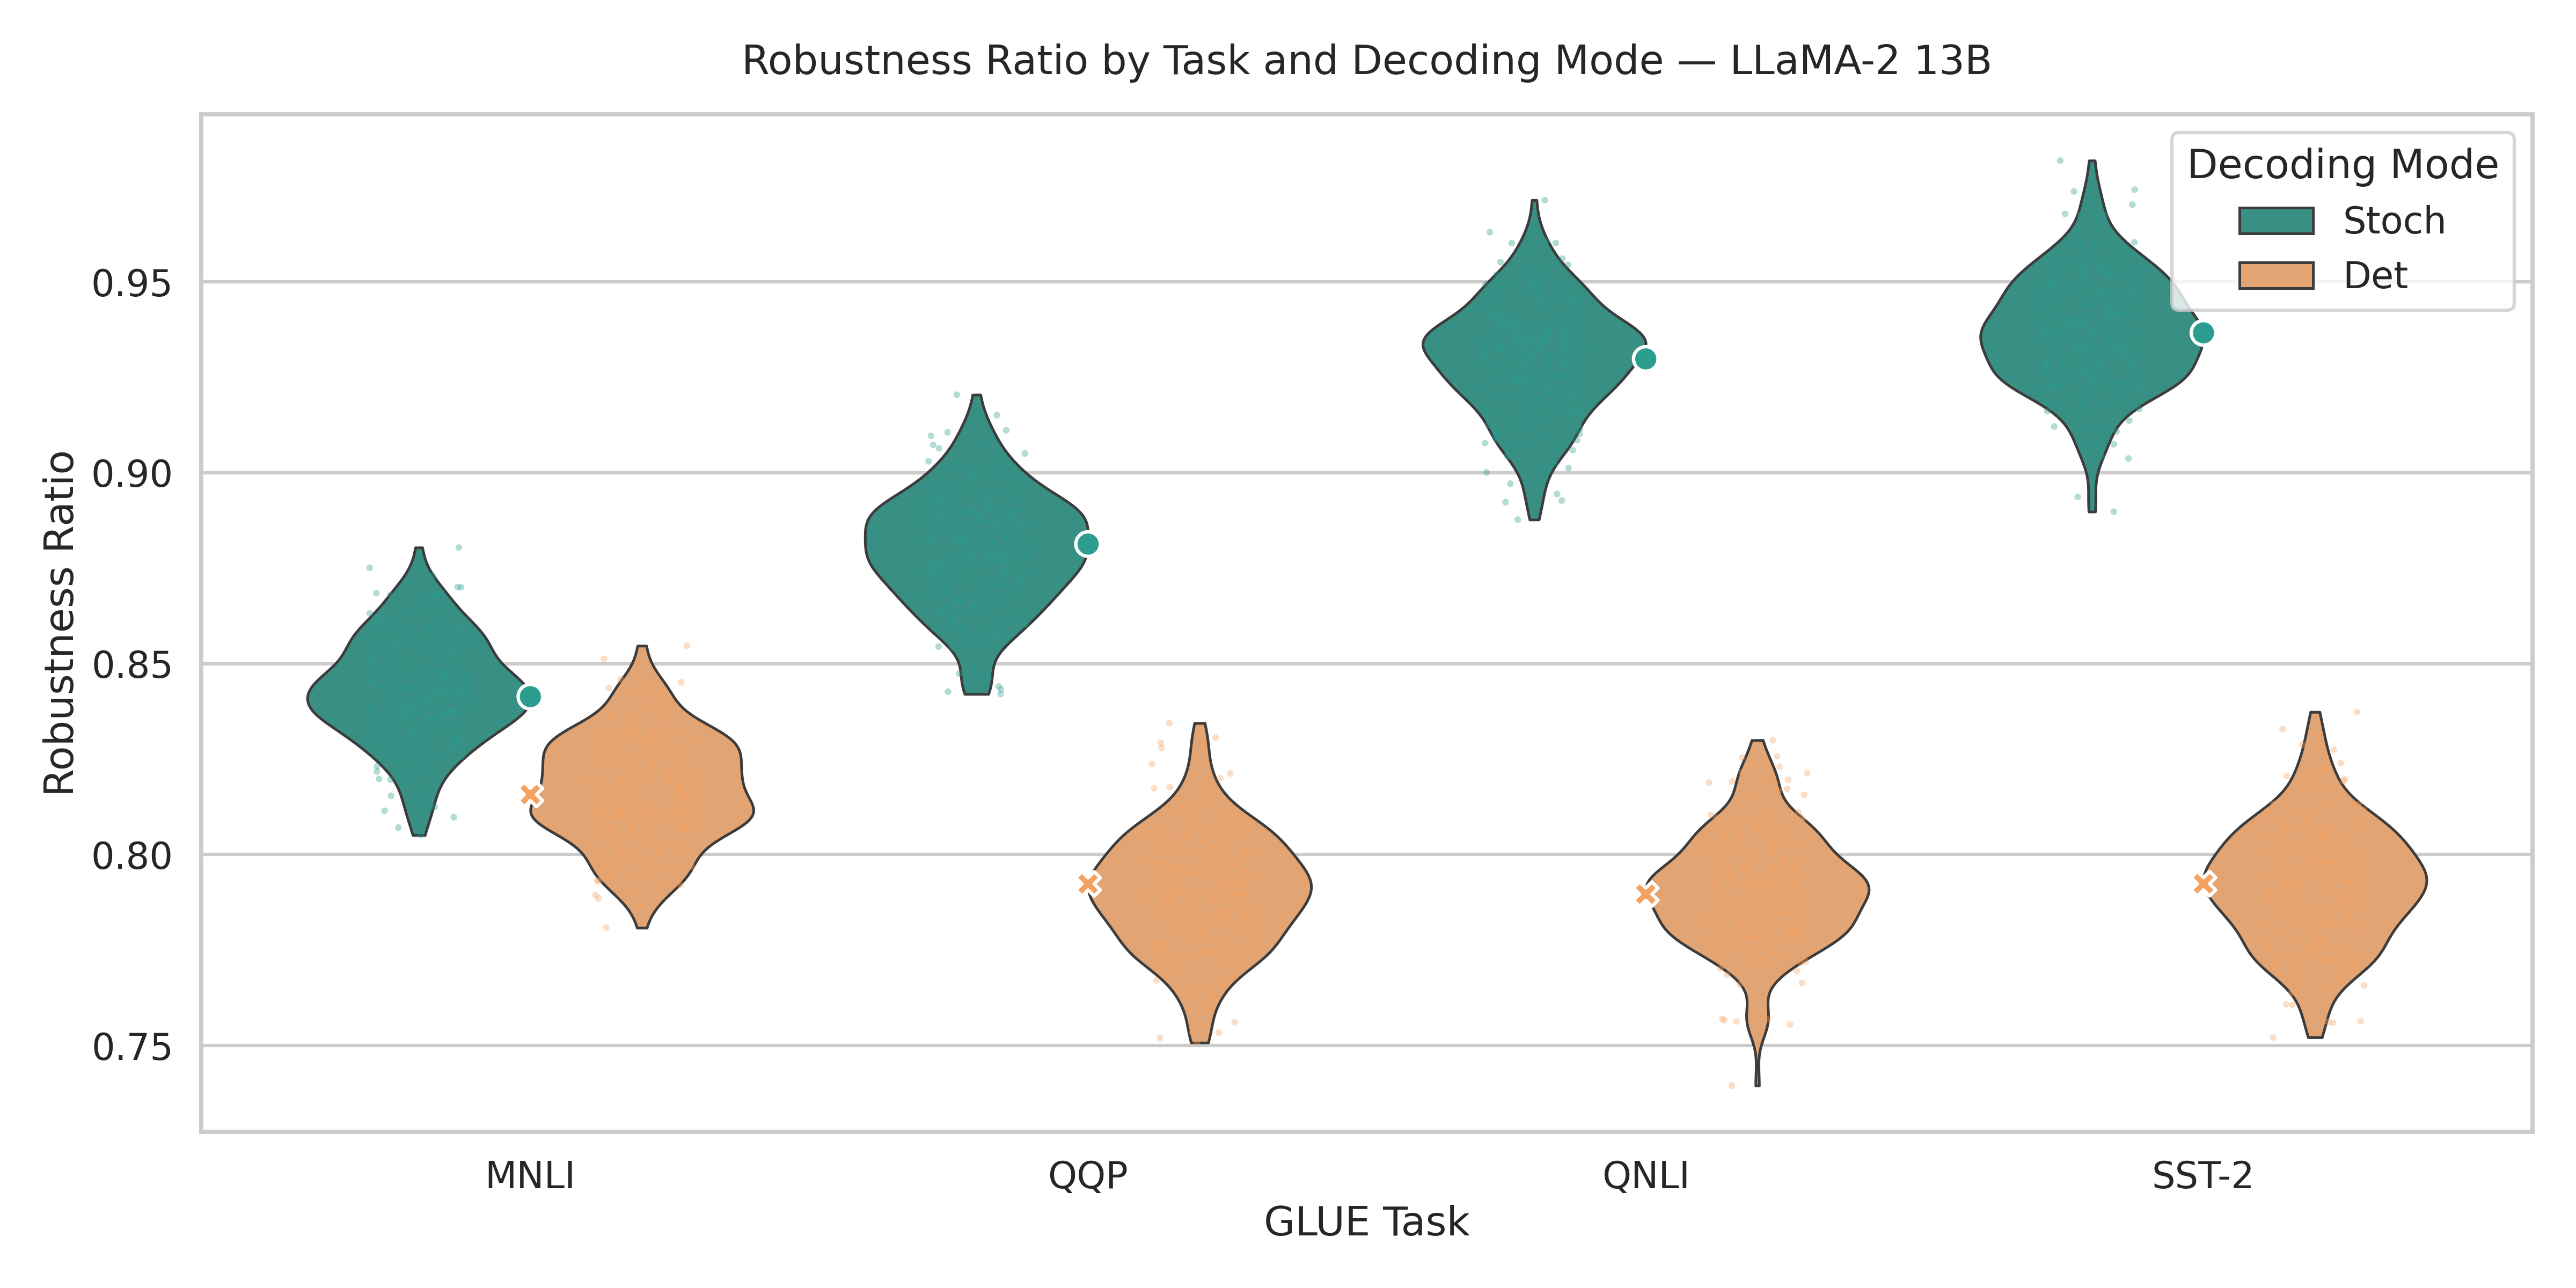
\includegraphics[width=\textwidth]{robustness_ratio/robustness_ratio_LLaMA-2_13B.png}
  \caption{
  \textbf{Robustness ratios for \emph{LLaMA-2 13B} across GLUE tasks.}
  After scaling to 13B, \textbf{stochastic robustness} climbs to the \(\mathbf{0.84\text{--}0.94}\) range, while \textbf{deterministic} decoding stays in a narrower but lower interval of \(\mathbf{0.79\text{--}0.82}\).
  The resulting stochastic–deterministic gaps fall between \(\mathbf{0.03}\) and \(\mathbf{0.14}\) absolute points, with the largest gains again on MNLI and QNLI.
  Compared to LLaMA-2 7B, both decoding modes shift upward and the stochastic violins become \textbf{tighter}, especially on QQP and SST-2.
  This figure shows that \emph{\textbf{scaling within the same family substantially improves robustness}}, yet the qualitative pattern remains: stochastic decoding consistently exposes a more robust operating regime than deterministic decoding.
  }
  \label{fig:robustness-llama2-13b}
\end{figure*}

\begin{figure*}[t]
  \centering
  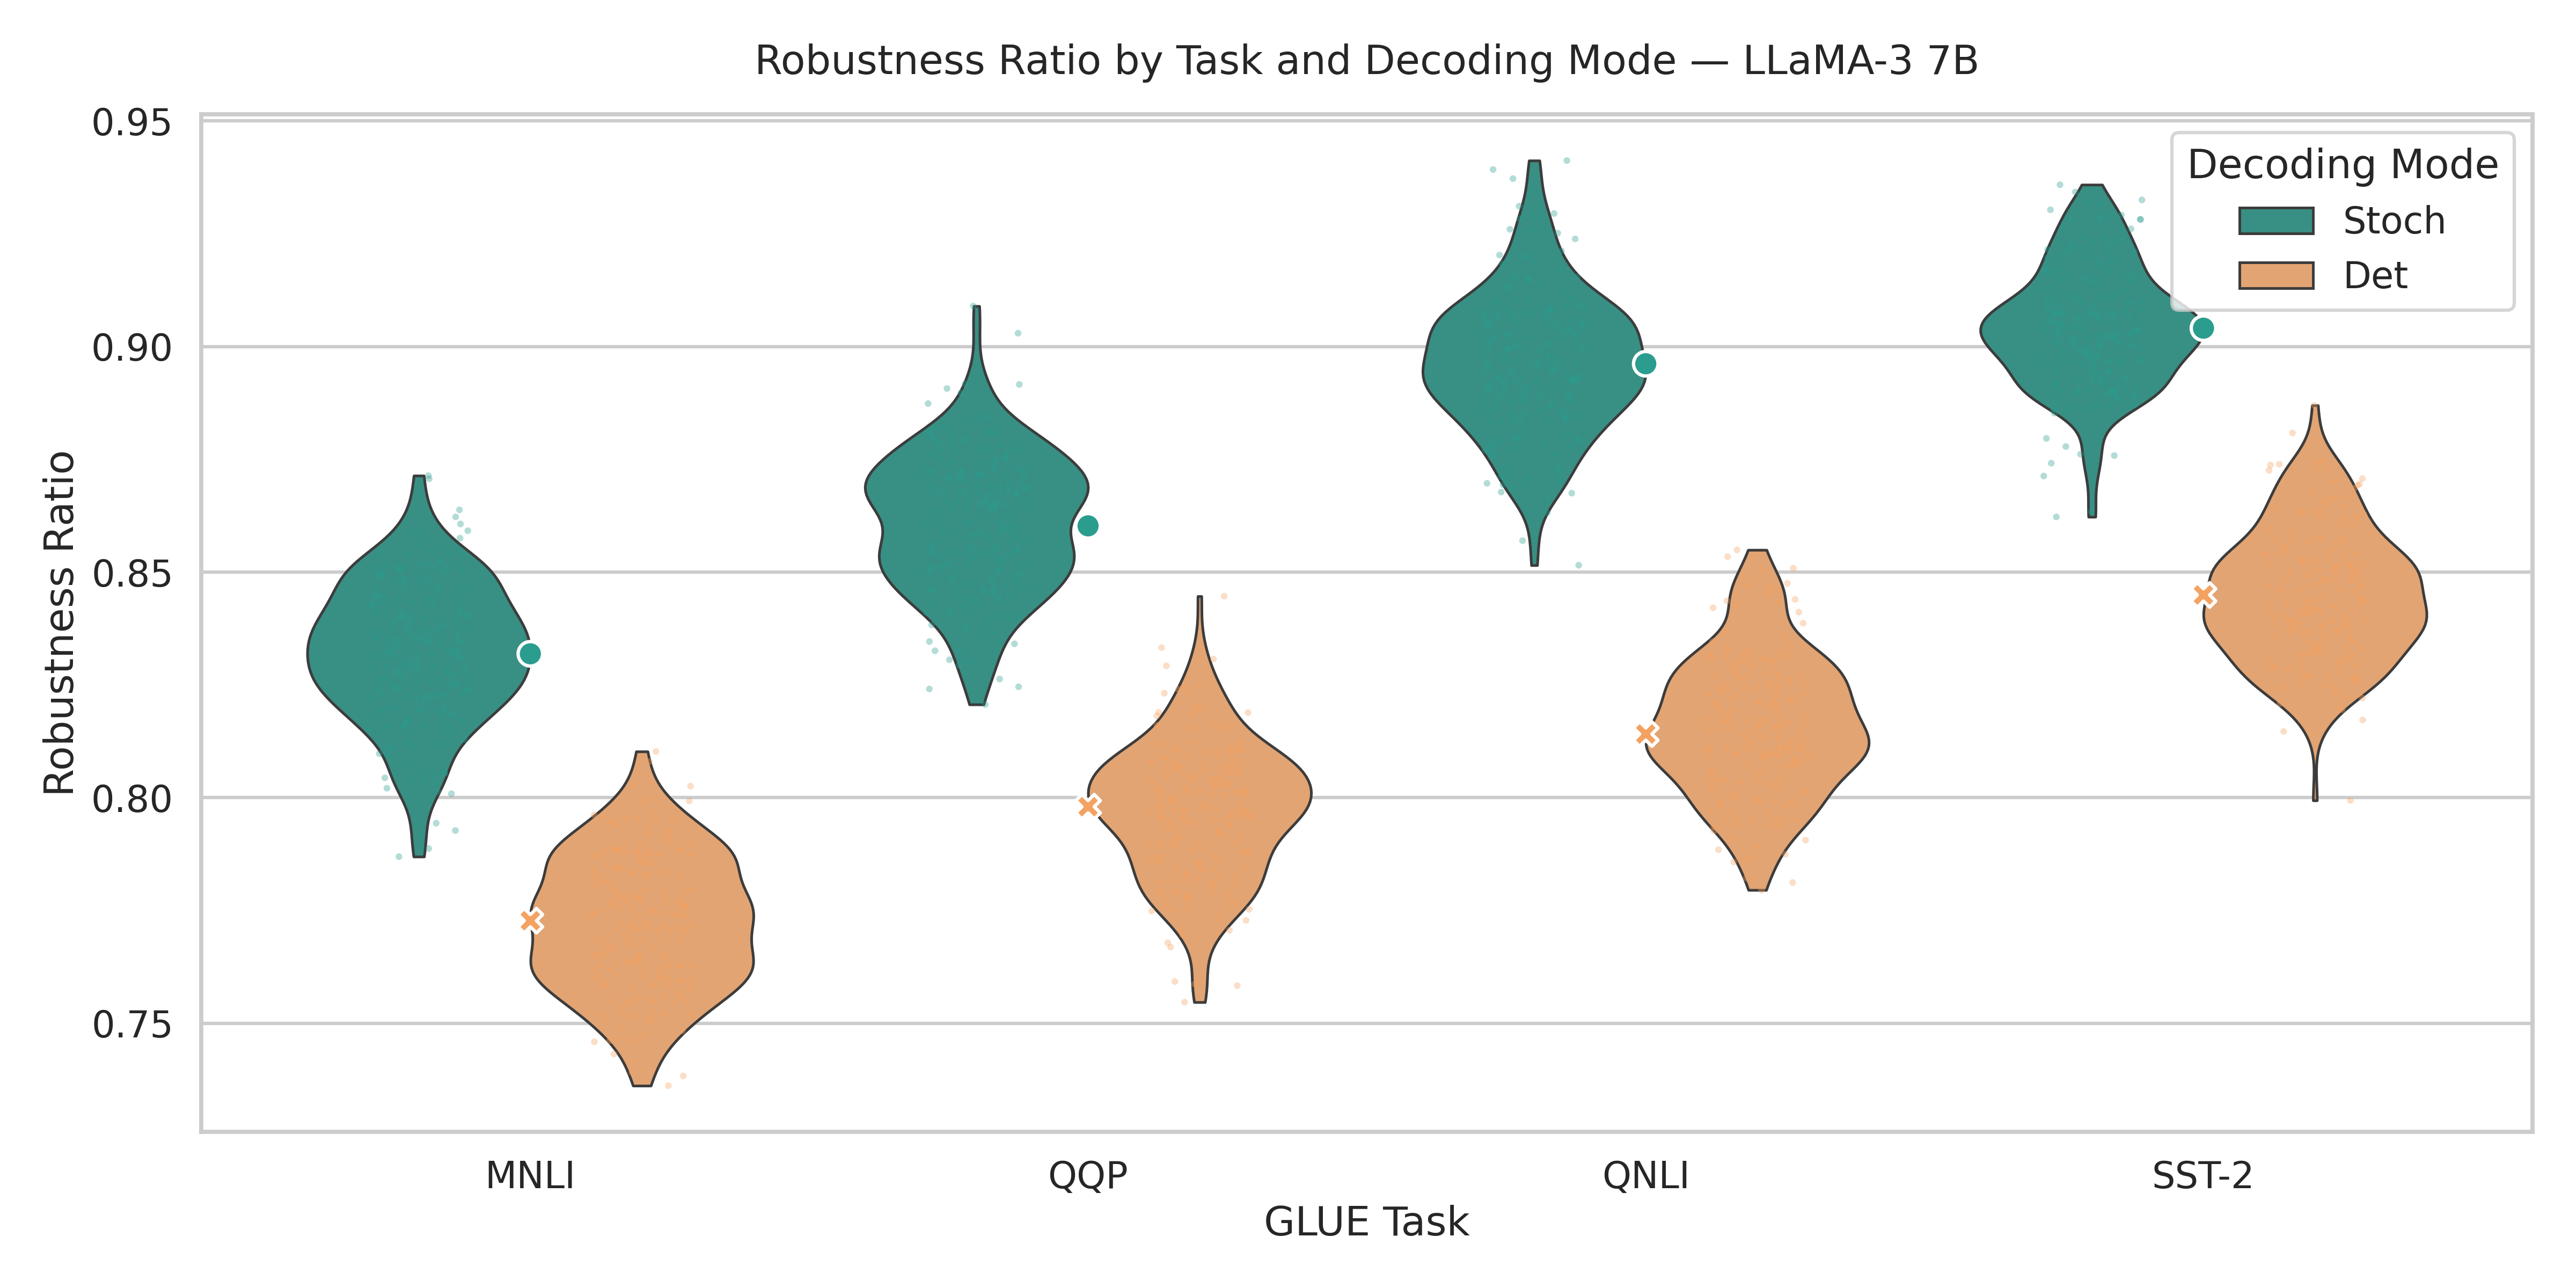
\includegraphics[width=\textwidth]{robustness_ratio/robustness_ratio_LLaMA-3_7B.png}
  \caption{
  \textbf{Robustness ratios for \emph{LLaMA-3 7B} across GLUE tasks.}
  Despite having the same parameter count as LLaMA-2 7B, \textbf{LLaMA-3 7B} achieves higher stochastic robustness, with ratios in the \(\mathbf{0.83\text{--}0.90}\) range.
  \textbf{Deterministic} decoding occupies \(\mathbf{0.77\text{--}0.84}\), and stochastic–deterministic gaps are more modest but still positive at roughly \(\mathbf{0.06\text{--}0.08}\) absolute points.
  QQP and QNLI show the \textbf{highest robustness and the tightest violins}, while MNLI remains the most challenging task.
  Quantitatively, this figure suggests that \emph{\textbf{architectural and data improvements from LLaMA-2 to LLaMA-3 shift the entire robustness band upward}}, even though the fundamental advantage of stochastic decoding persists.
  }
  \label{fig:robustness-llama3-7b}
\end{figure*}


\begin{figure*}[t]
  \centering
  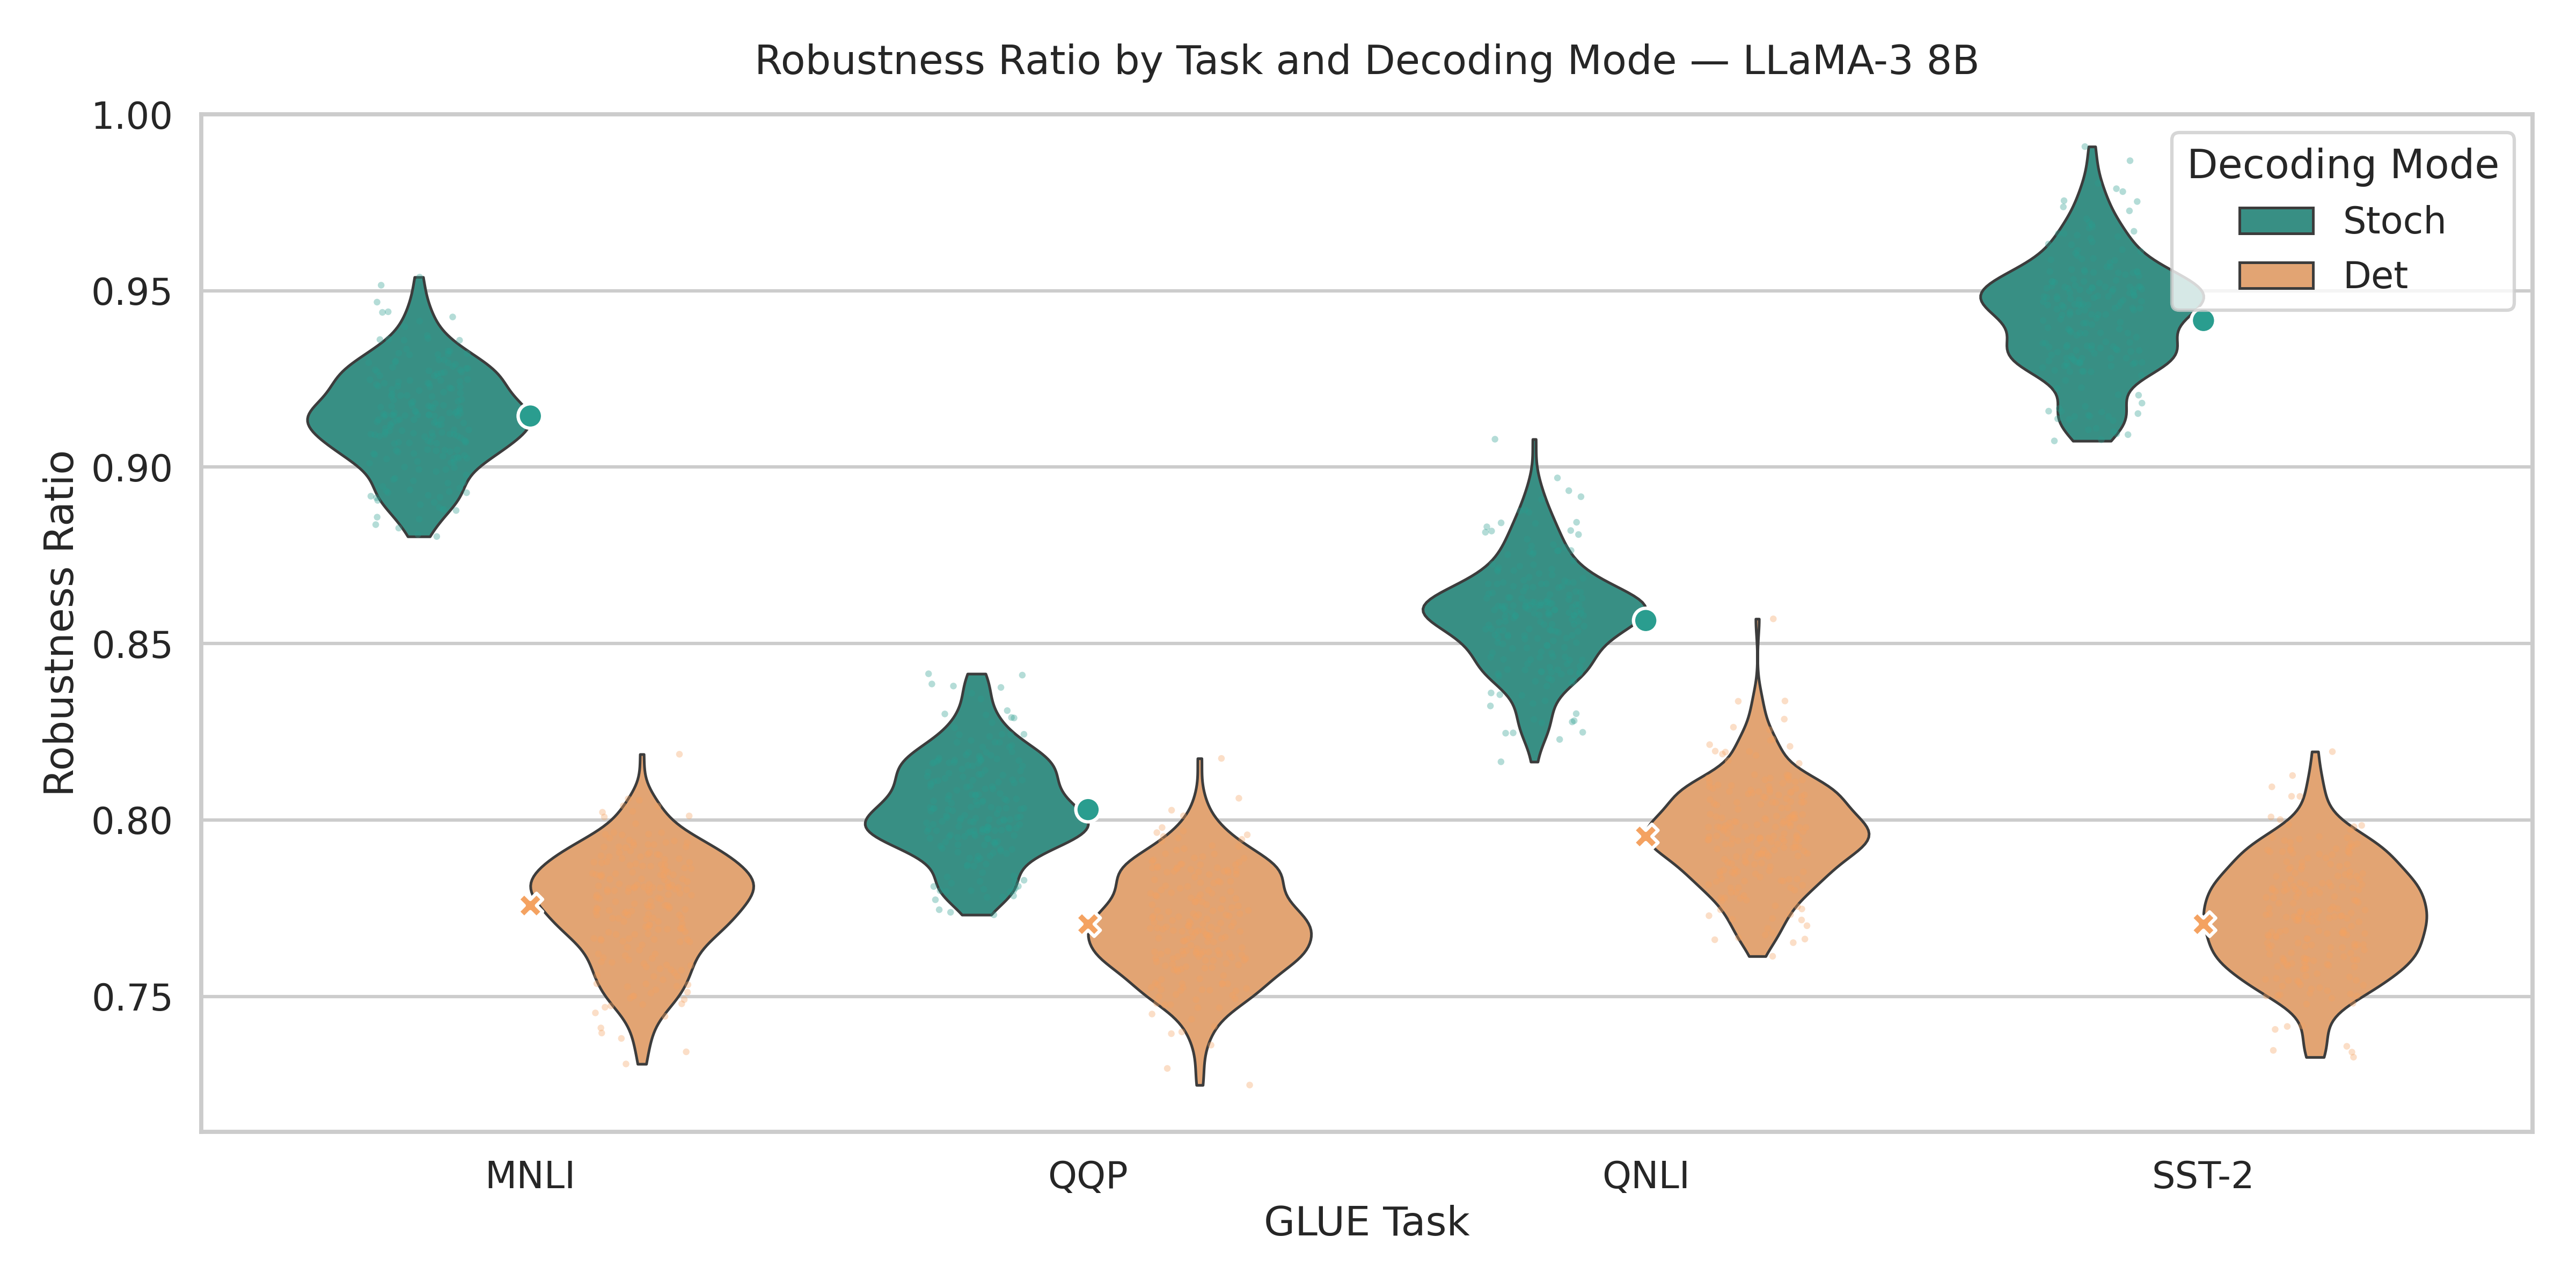
\includegraphics[width=\textwidth]{robustness_ratio/robustness_ratio_LLaMA-3_8B.png}
  \caption{
  \textbf{Robustness ratios for \emph{LLaMA-3 8B} across GLUE tasks.}
  Under \textbf{stochastic decoding}, LLaMA-3 8B attains robustness ratios in the \(\mathbf{0.89\text{--}0.96}\) band (roughly \(\mathbf{0.91}\) on MNLI, \(\mathbf{0.80}\) on QQP, \(\mathbf{0.86}\) on QNLI, and \(\mathbf{0.95}\) on SST-2), whereas \textbf{deterministic decoding} falls to the \(\mathbf{0.74\text{--}0.79}\) band across the same tasks.
  The stochastic–deterministic gaps range from about \(\mathbf{0.06}\) (QQP, QNLI) up to nearly \(\mathbf{0.18}\) (SST-2), showing \textbf{large decoding-induced robustness gains}.
  The high, tight stochastic violin on SST-2 in particular indicates that \emph{\textbf{LLaMA-3 8B becomes extremely robust when decoded stochastically}}, while deterministic decoding systematically underestimates its robustness.
  }
  \label{fig:robustness-llama3-8b}
\end{figure*}

\begin{figure*}[t]
  \centering
  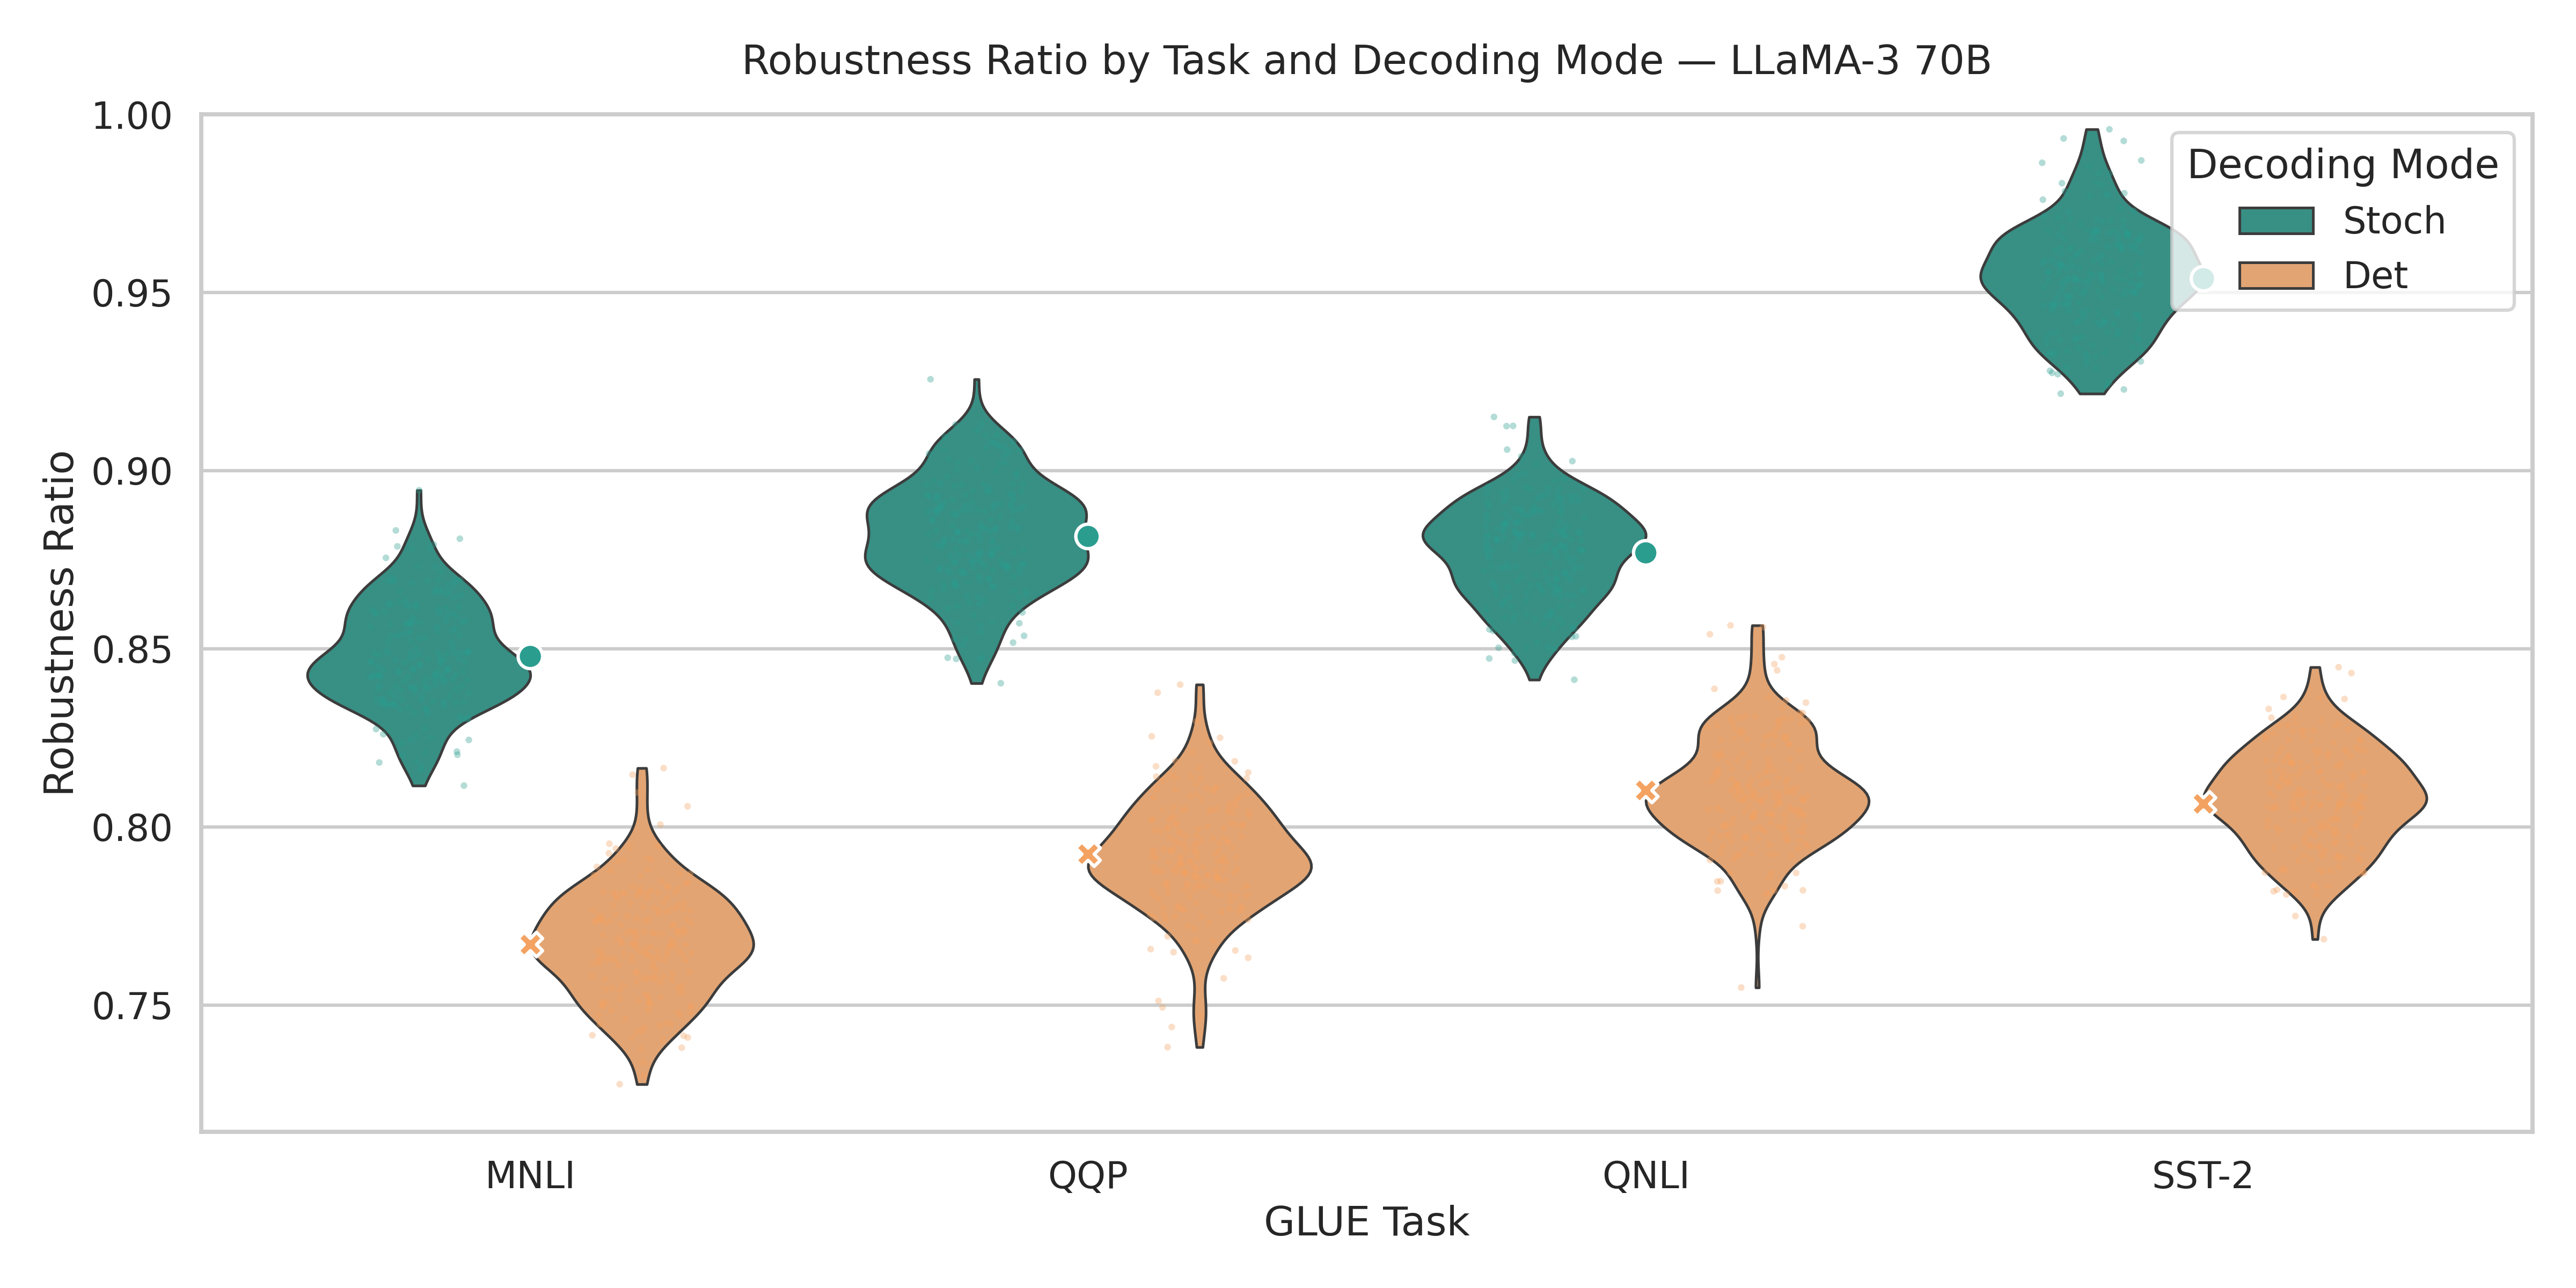
\includegraphics[width=\textwidth]{robustness_ratio/robustness_ratio_LLaMA-3_70B.png}
  \caption{
  \textbf{Robustness ratios for \emph{LLaMA-3 70B} across GLUE tasks.}
  \textbf{Stochastic decoding} places LLaMA-3 70B in a strong robustness band of \(\mathbf{0.84\text{--}0.96}\): around \(\mathbf{0.85}\) on MNLI, \(\mathbf{0.88}\) on QQP, \(\mathbf{0.88}\) on QNLI, and near \(\mathbf{0.96}\) on SST-2.
  In contrast, \textbf{deterministic decoding} compresses robustness into the lower \(\mathbf{0.74\text{--}0.83}\) interval.
  The resulting stochastic–deterministic differences span roughly \(\mathbf{0.04\text{--}0.13}\) absolute points, with the \textbf{largest margins on SST-2 and QQP}.
  Compared with LLaMA-3 7B, these numbers show that \emph{\textbf{scaling to 70B significantly strengthens robustness while preserving the same qualitative advantage of stochastic decoding}}.
  }
  \label{fig:robustness-llama3-70b}
\end{figure*}

\begin{figure*}[t]
  \centering
  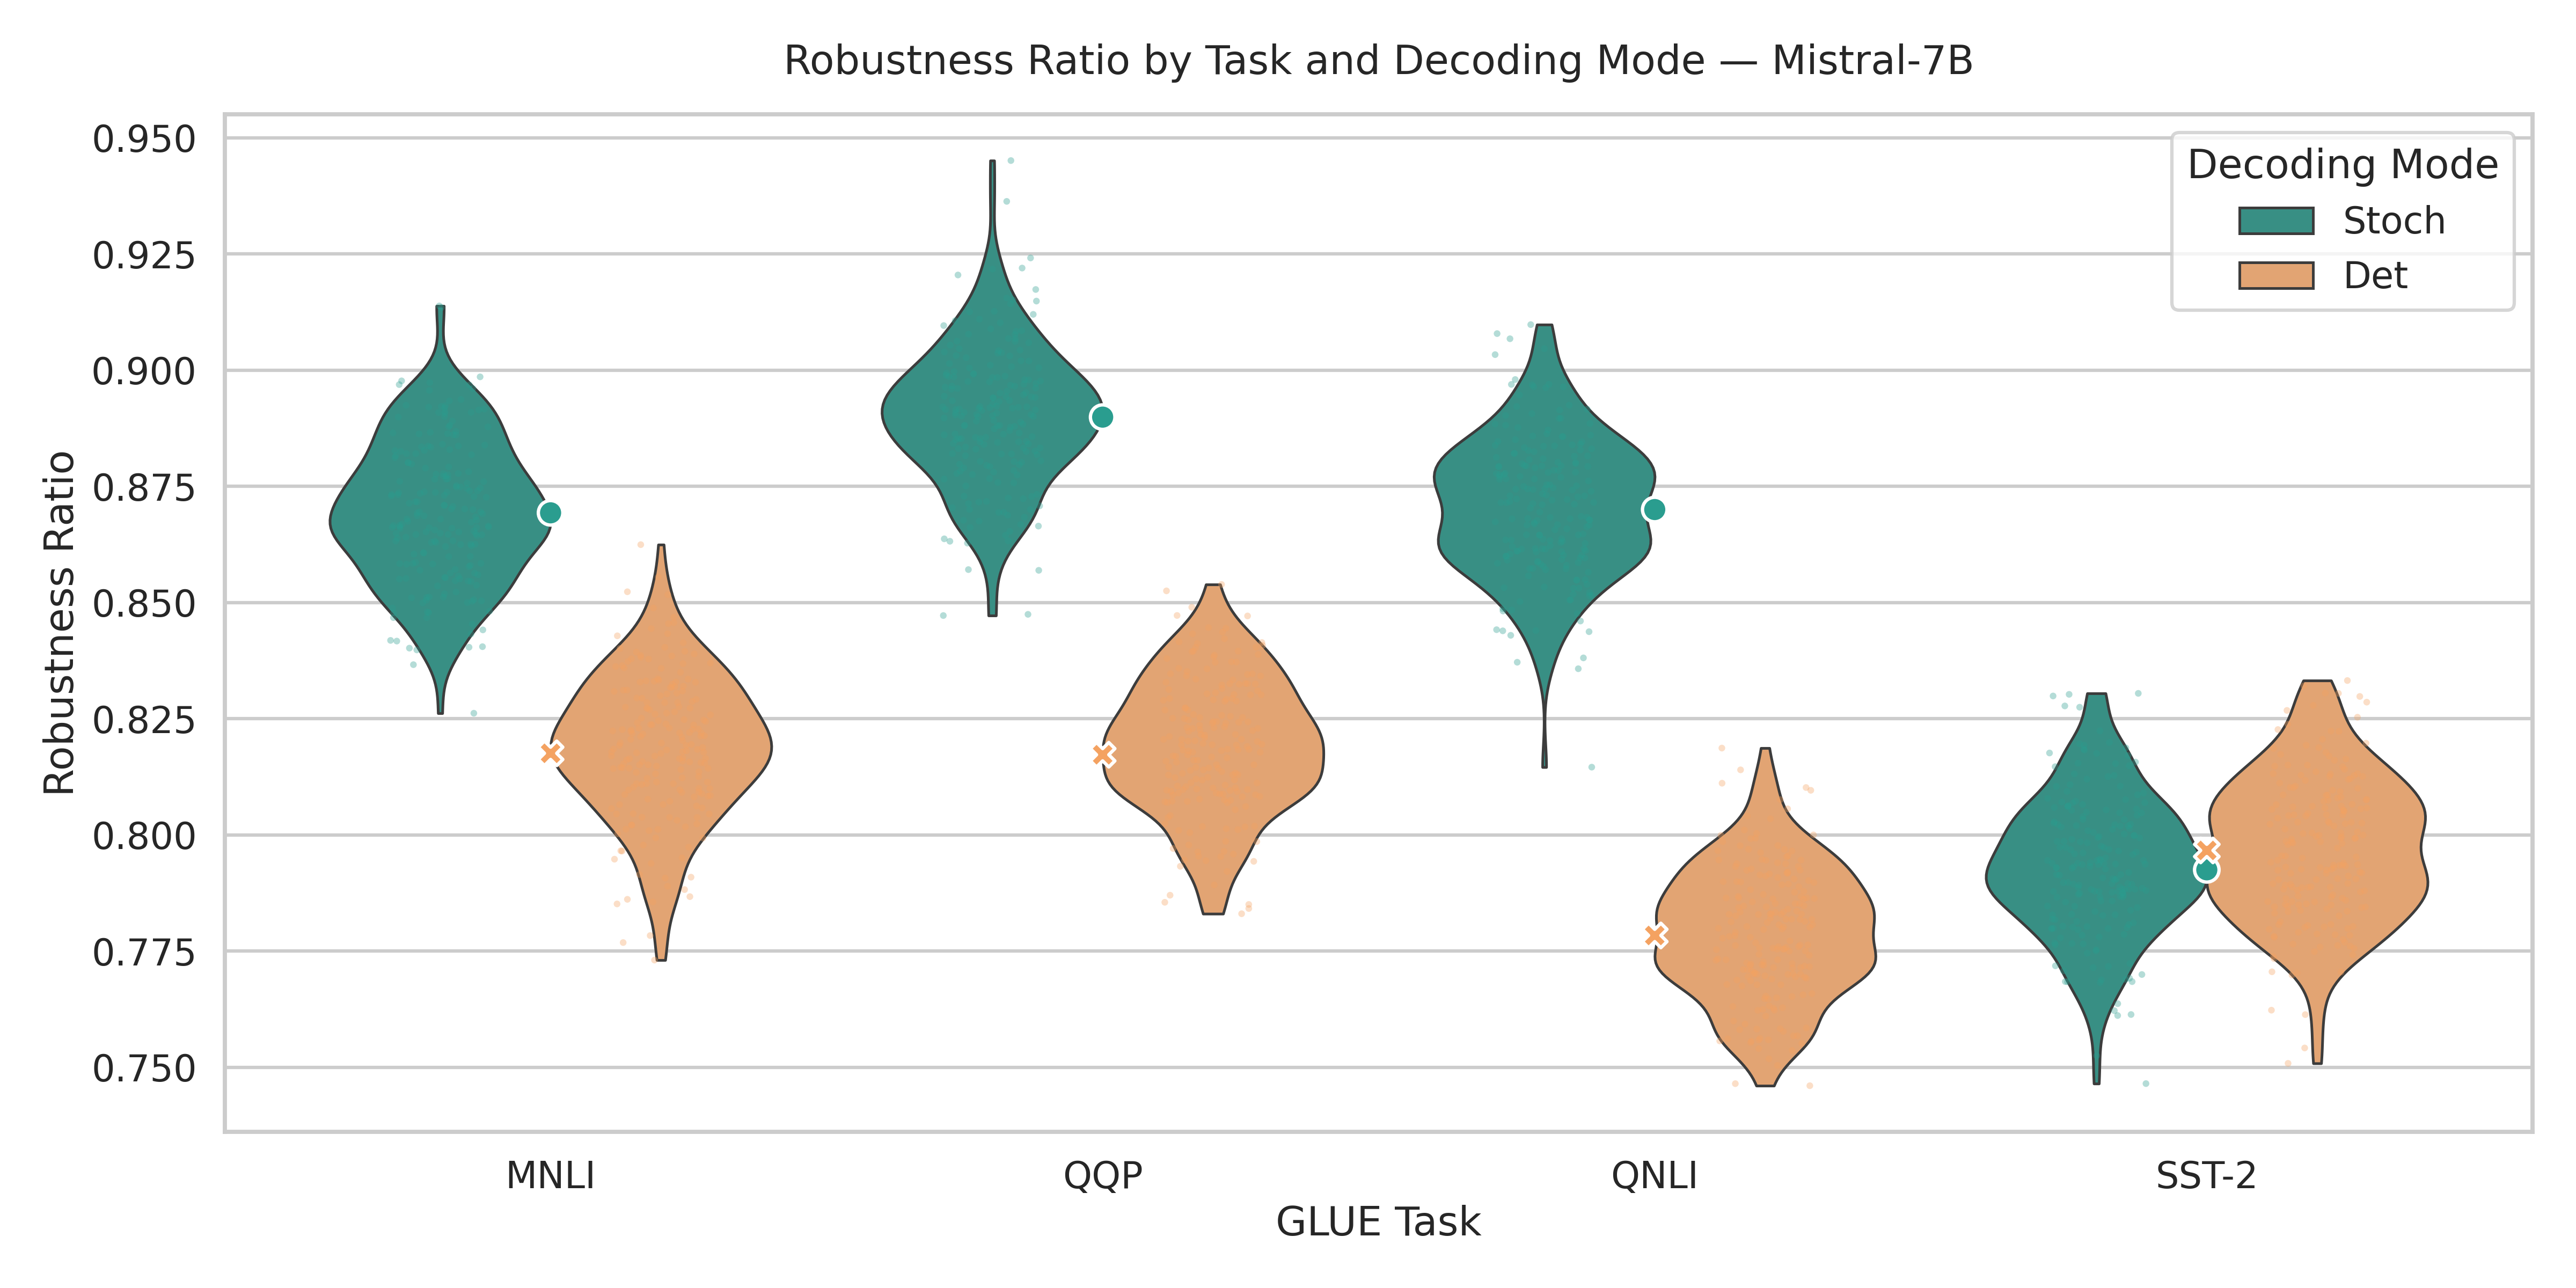
\includegraphics[width=\textwidth]{robustness_ratio/robustness_ratio_Mistral-7B.png}
  \caption{
  \textbf{Robustness ratios for \emph{Mistral-7B} across GLUE tasks.}
  With \textbf{stochastic} decoding, Mistral-7B achieves robustness ratios between \(\mathbf{0.84}\) and \(\mathbf{0.90}\) on MNLI, QQP, and QNLI, and around \(\mathbf{0.78\text{--}0.82}\) on SST-2.
  \textbf{Deterministic} decoding yields slightly lower values on most tasks, in the \(\mathbf{0.79\text{--}0.84}\) range for MNLI/QQP/QNLI and around \(\mathbf{0.77\text{--}0.82}\) on SST-2.
  Stochastic–deterministic gaps are moderate (\(\mathbf{0.02\text{--}0.06}\) absolute), except for SST-2 where deterministic decoding is marginally higher, illustrating that \textbf{the decoding advantage can flip on specific tasks}.
  Overall, the figure highlights that \emph{\textbf{Mistral-7B is reasonably robust but exhibits nuanced, task-specific trade-offs between stochastic and deterministic decoding}}.
  }
  \label{fig:robustness-mistral7b}
\end{figure*}

\begin{figure*}[t]
  \centering
  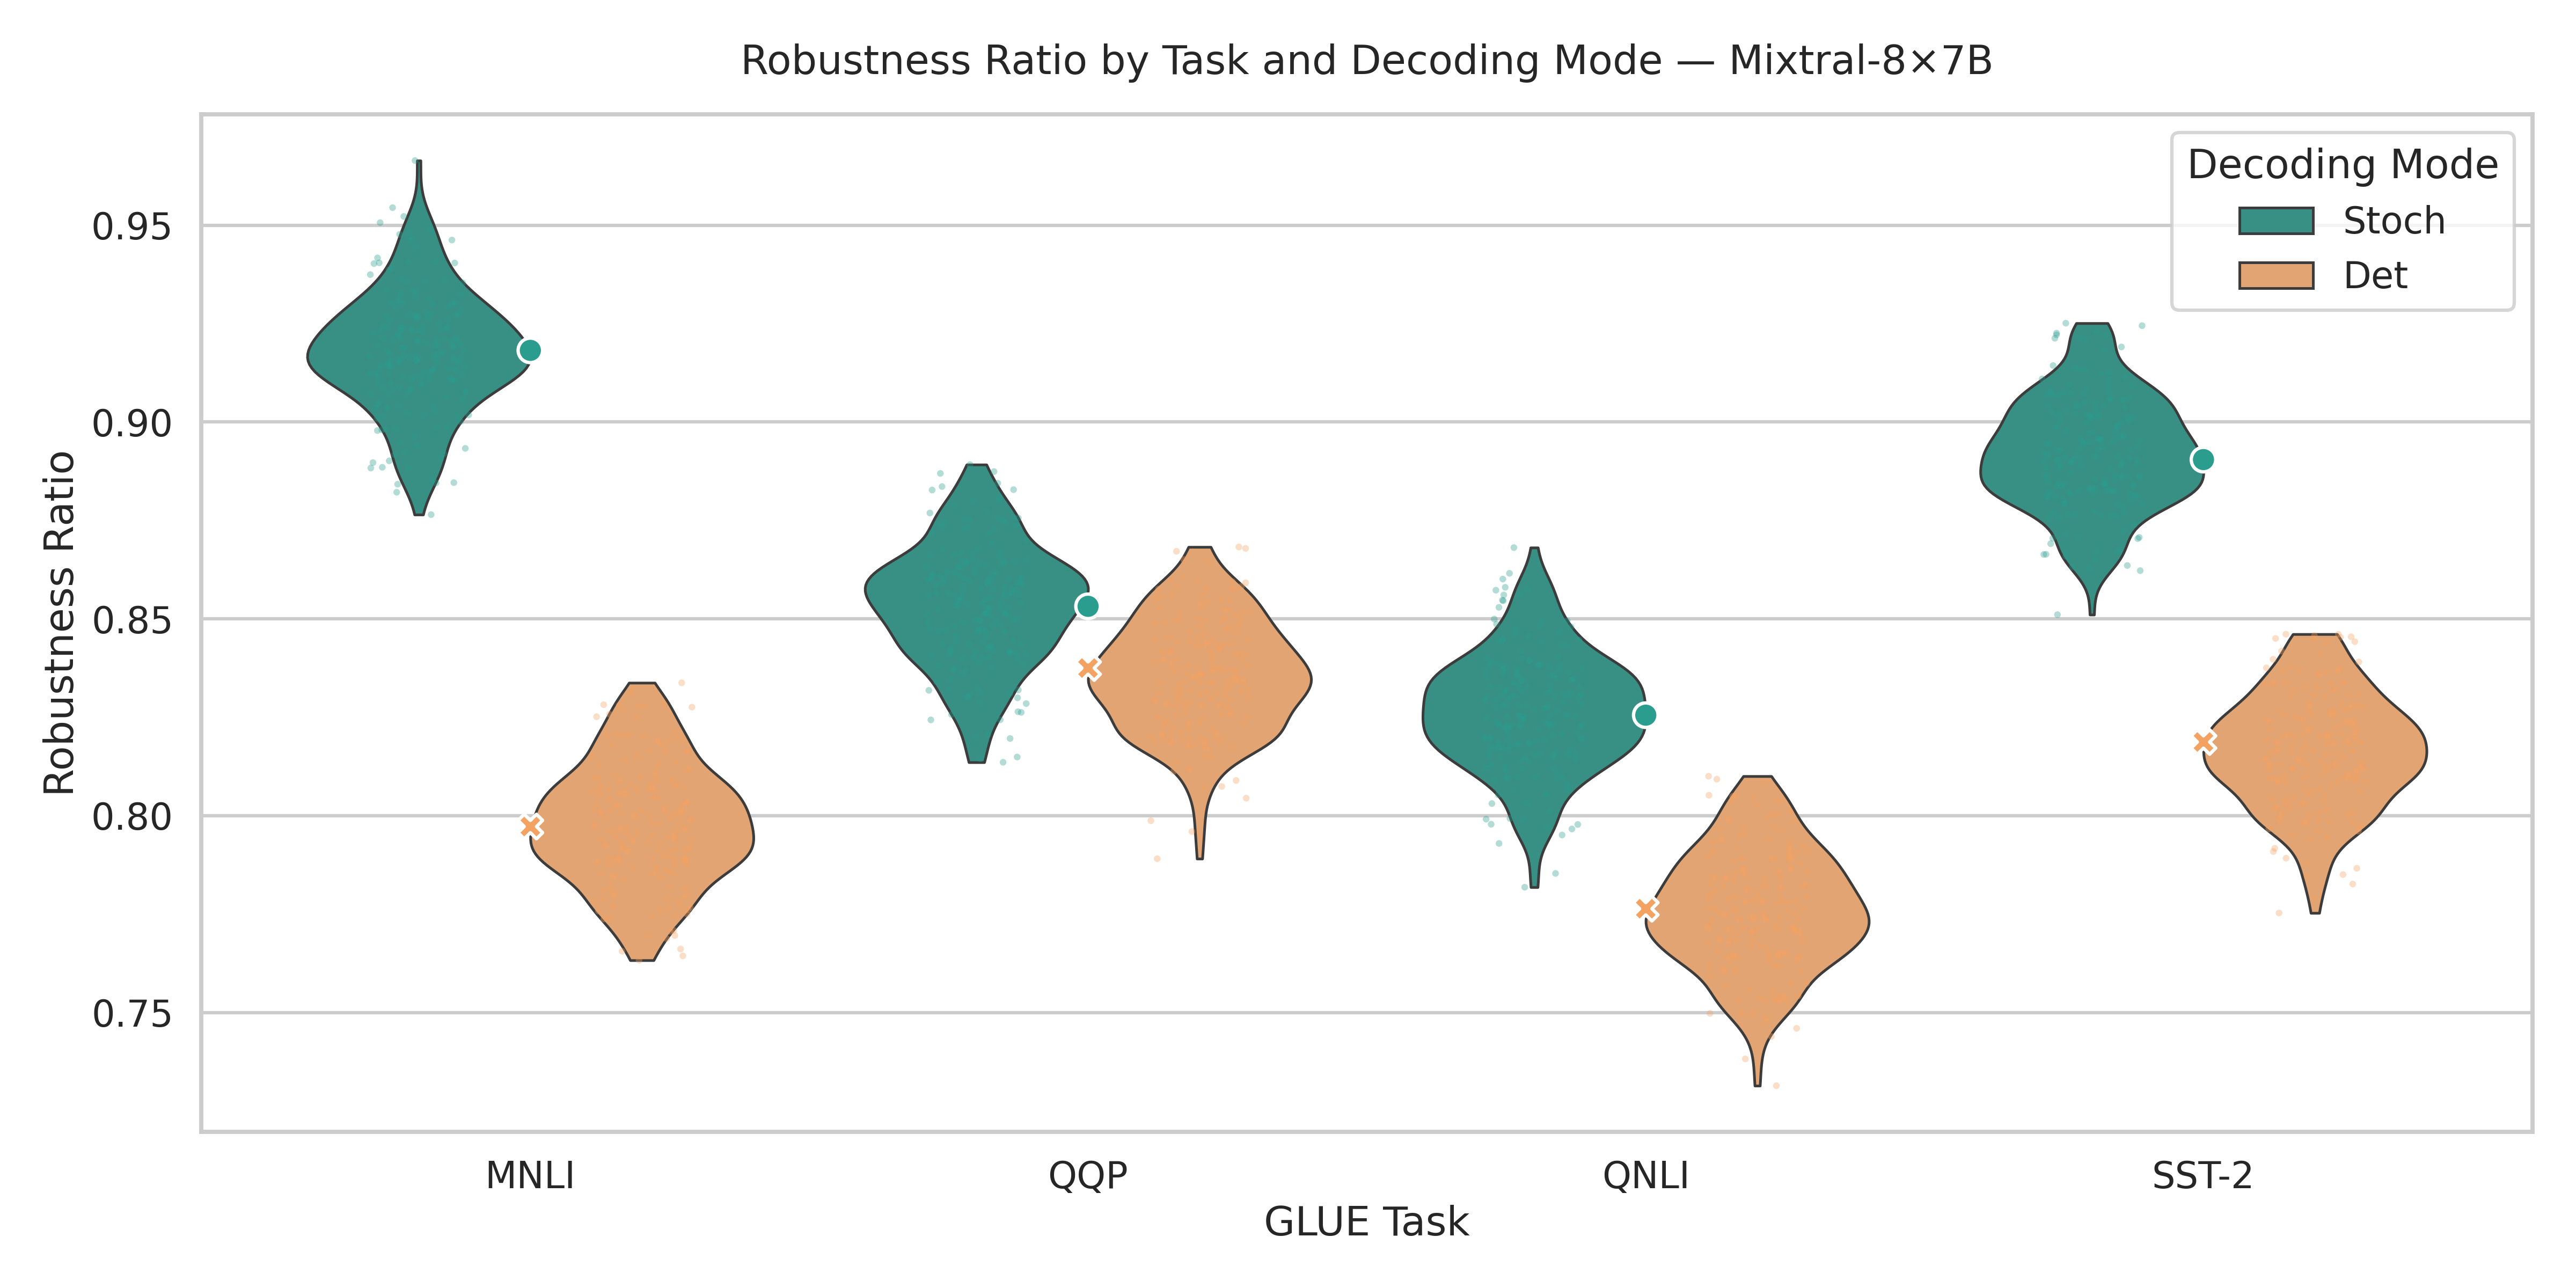
\includegraphics[width=\textwidth]{robustness_ratio/robustness_ratio_Mixtral-8x7B.png}
  \caption{
  \textbf{Robustness ratios for \emph{Mixtral-8$\times$7B} across GLUE tasks.}
  \textbf{Stochastic decoding} places the mixture-of-experts model in a high band of \(\mathbf{0.83\text{--}0.95}\): about \(\mathbf{0.92}\) on MNLI, \(\mathbf{0.86}\) on QQP, \(\mathbf{0.83}\) on QNLI, and \(\mathbf{0.89}\) on SST-2.
  \textbf{Deterministic decoding} yields \(\mathbf{0.77\text{--}0.84}\) across tasks, often trailing stochastic decoding by \(\mathbf{0.05\text{--}0.10}\) absolute points.
  The largest gaps appear on MNLI and SST-2, where violins are clearly separated, while QQP shows a smaller but still positive advantage for stochastic decoding.
  These patterns indicate that \emph{\textbf{routing-based models like Mixtral-8$\times$7B can be highly robust, but their robustness is substantially unlocked only under stochastic inference}}.
  }
  \label{fig:robustness-mixtral-8x7b}
\end{figure*}

\begin{figure*}[t]
  \centering
  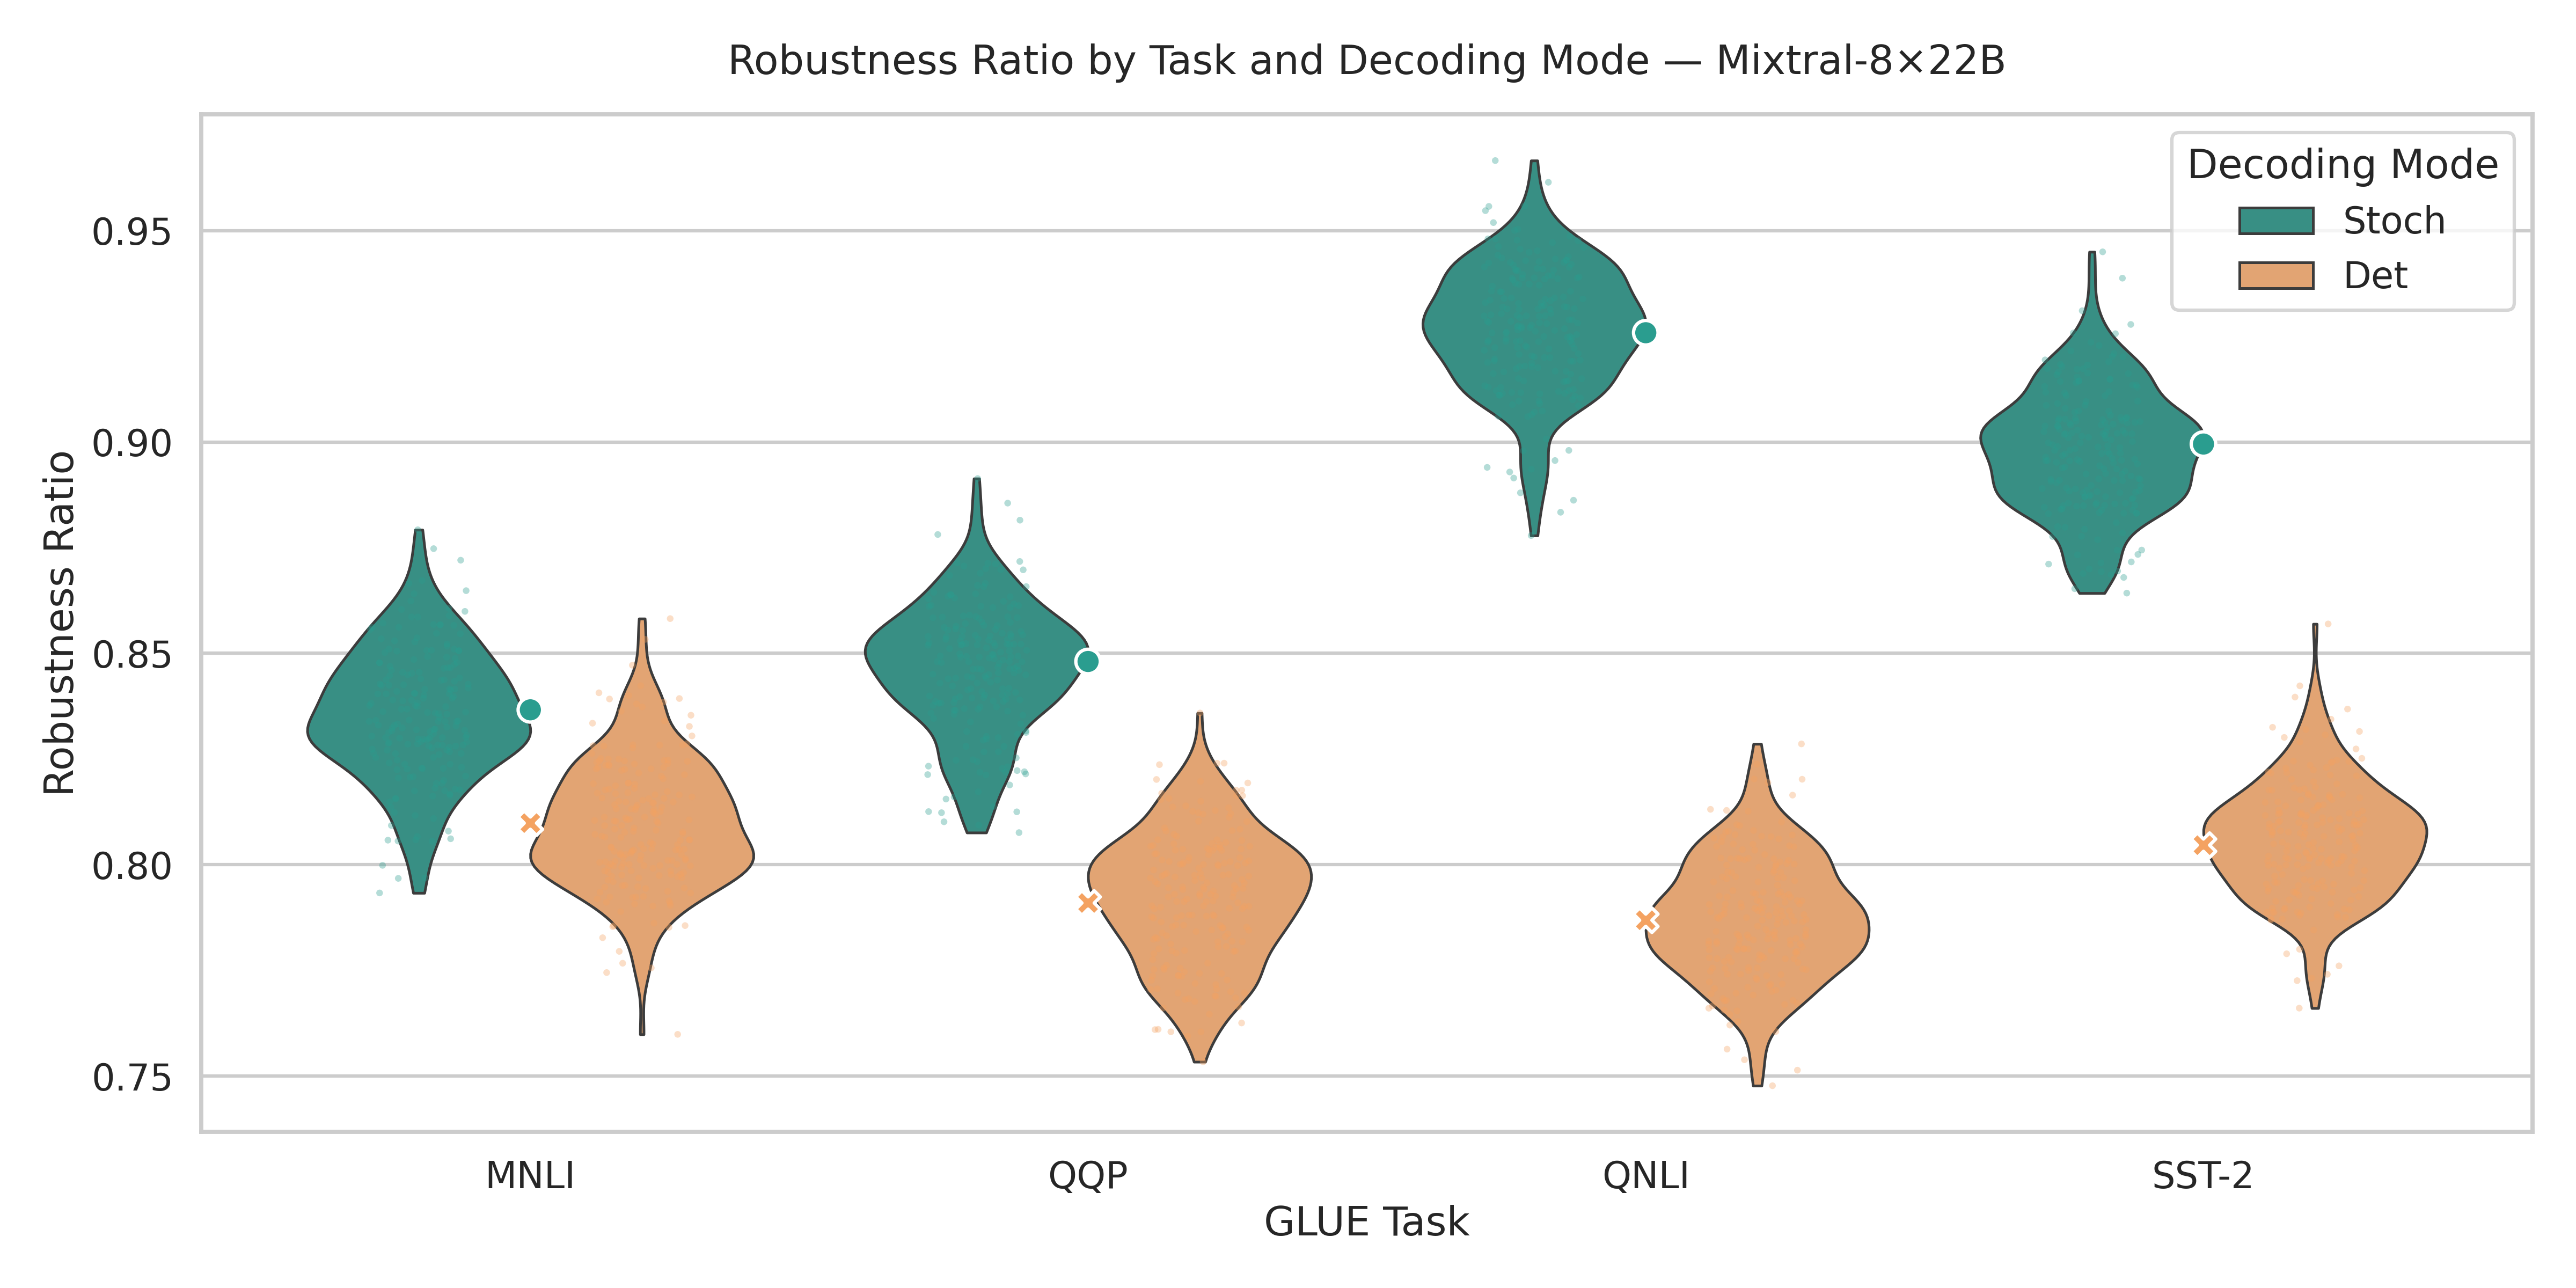
\includegraphics[width=\textwidth]{robustness_ratio/robustness_ratio_Mixtral-8x22B.png}
  \caption{
  \textbf{Robustness ratios for \emph{Mixtral-8$\times$22B} across GLUE tasks.}
  Scaling Mixtral to \textbf{8$\times$22B} yields stochastic robustness ratios in the \(\mathbf{0.84\text{--}0.95}\) band: about \(\mathbf{0.84}\) on MNLI, \(\mathbf{0.85}\) on QQP, \(\mathbf{0.93}\) on QNLI, and \(\mathbf{0.90}\) on SST-2.
  \textbf{Deterministic decoding} remains in a lower \(\mathbf{0.78\text{--}0.82}\) band across all tasks.
  The stochastic–deterministic margins are modest (\(\mathbf{0.03\text{--}0.06}\)) on MNLI/QQP/SST-2 but become very large on QNLI (\(\approx\mathbf{0.10\text{--}0.15}\)).
  The very tall, narrow stochastic violin for QNLI emphasizes \textbf{high and stable robustness}, whereas deterministic decoding exhibits both lower means and larger spread.
  Thus, \emph{\textbf{Mixtral-8$\times$22B combines scale with strong stochastic robustness, particularly on inference-style QNLI}}.
  }
  \label{fig:robustness-mixtral-8x22b}
\end{figure*}

\begin{figure*}[t]
  \centering
  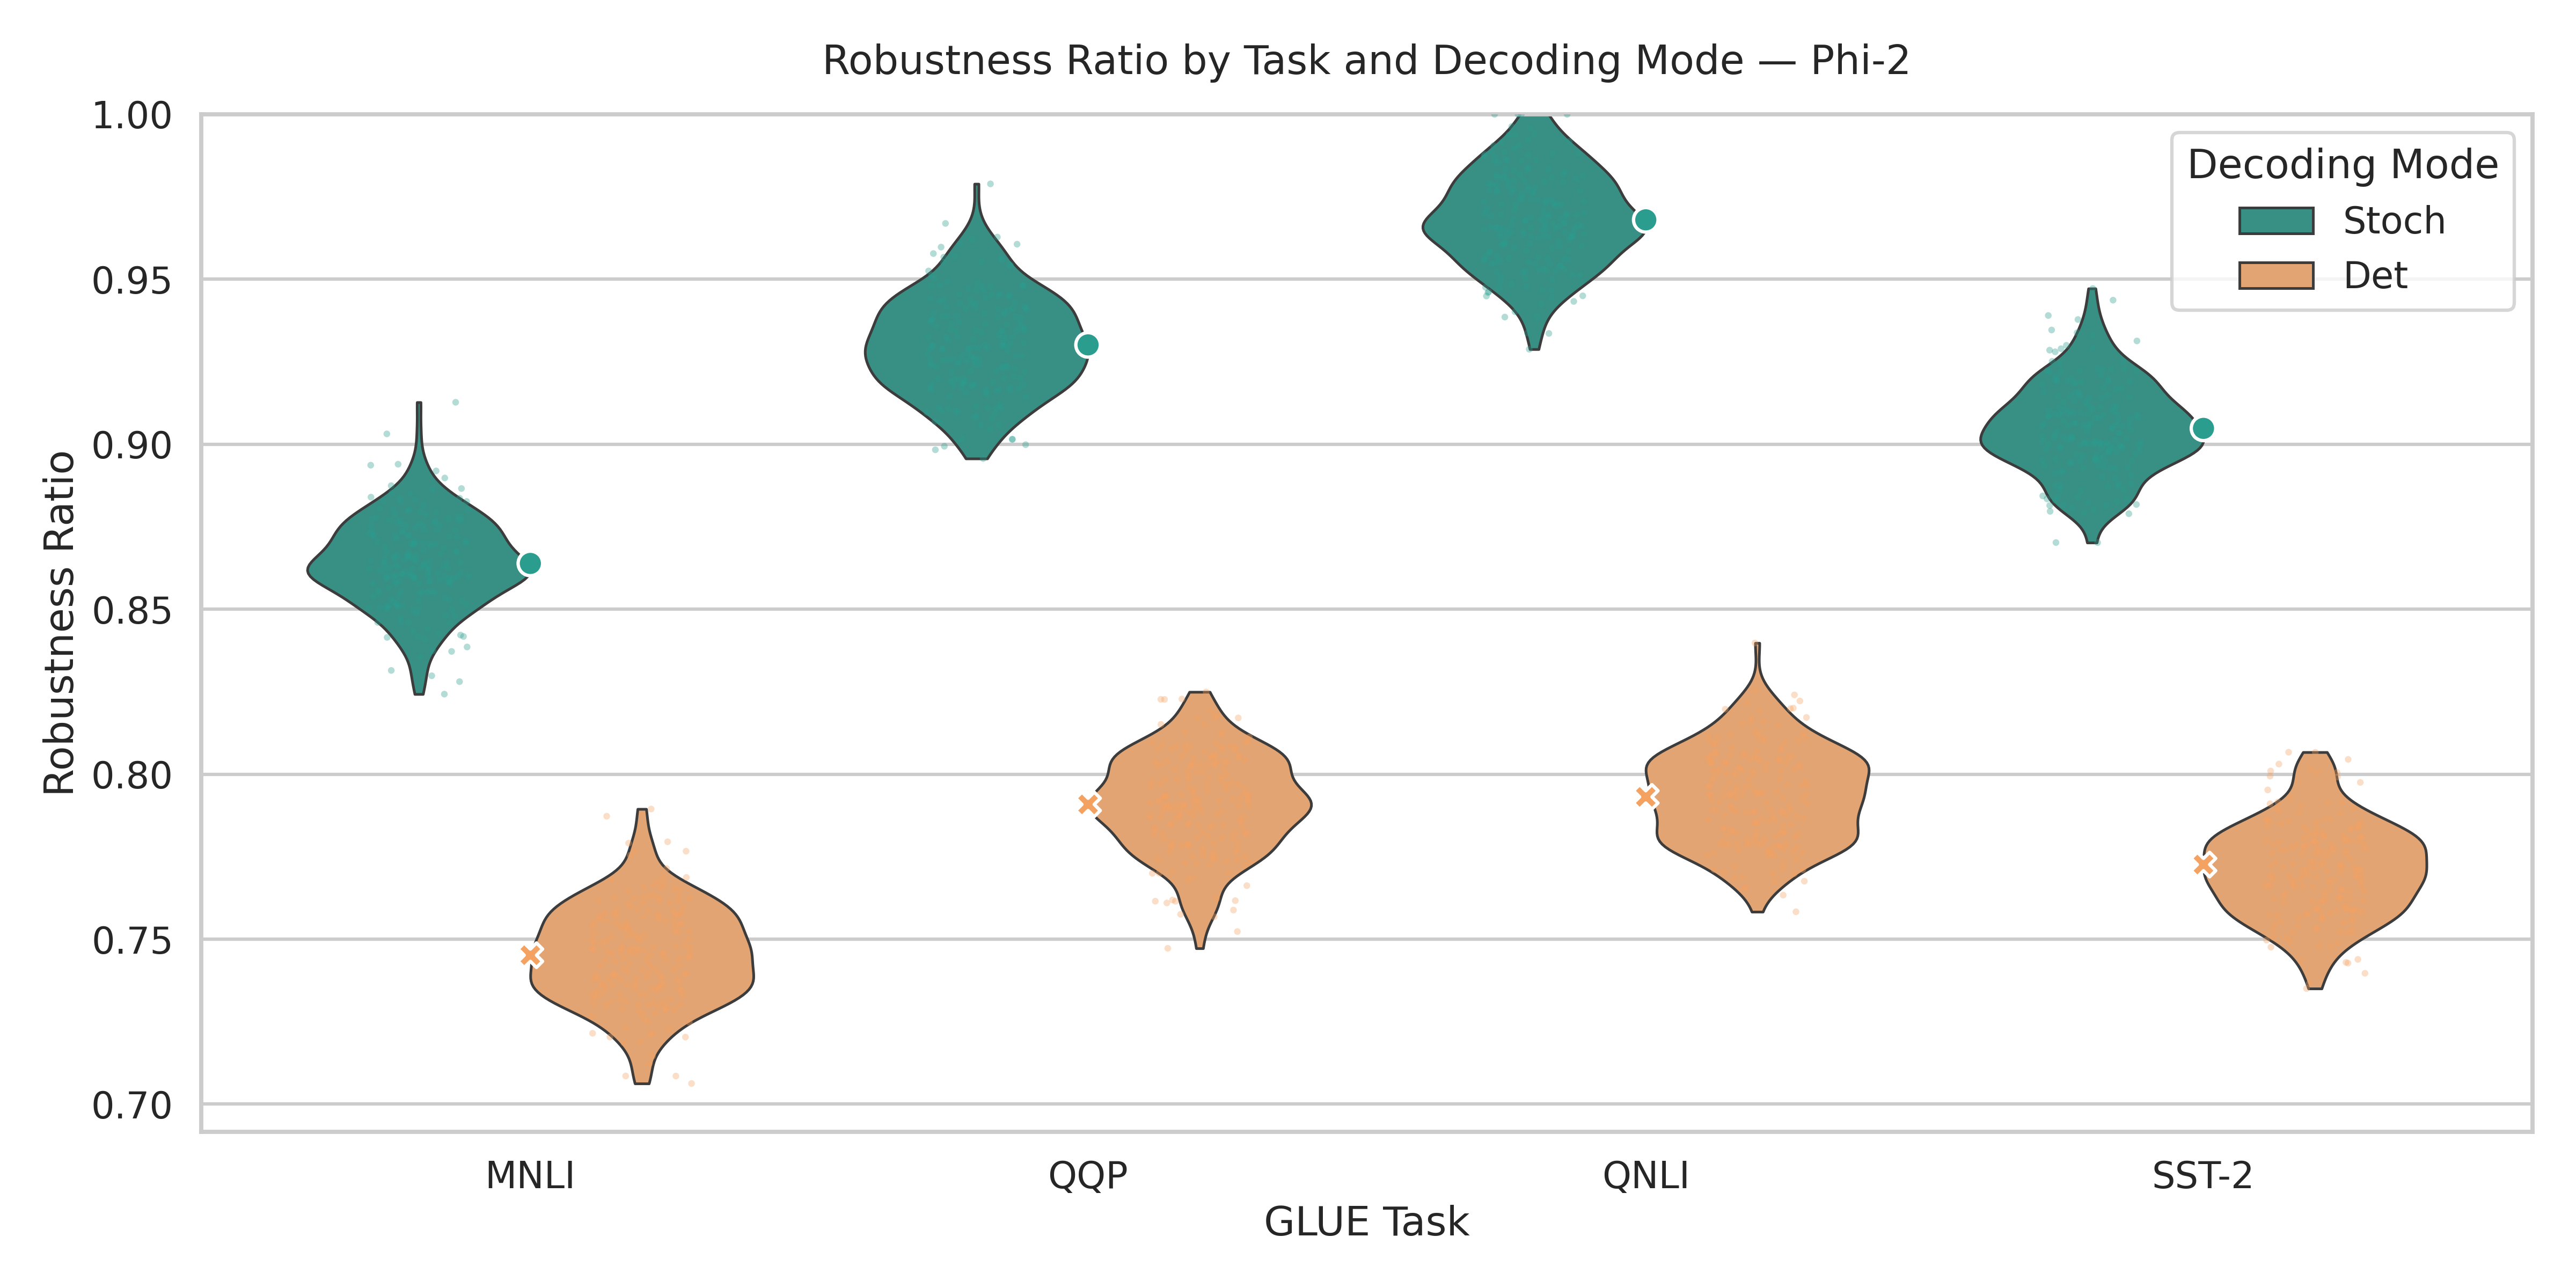
\includegraphics[width=\textwidth]{robustness_ratio/robustness_ratio_Phi-2.png}
  \caption{
  \textbf{Robustness ratios for \emph{Phi-2} across GLUE tasks.}
  Despite being a small model, \textbf{stochastic decoding} propels Phi-2 to surprisingly high robustness ratios: around \(\mathbf{0.86}\) on MNLI, \(\mathbf{0.93\text{--}0.95}\) on QQP, \(\mathbf{0.96\text{--}0.98}\) on QNLI, and \(\mathbf{0.89\text{--}0.93}\) on SST-2.
  In contrast, \textbf{deterministic decoding} stays in the \(\mathbf{0.74\text{--}0.80}\) band across tasks.
  This yields very large stochastic–deterministic gaps of roughly \(\mathbf{0.10\text{--}0.17}\) absolute points, some of the \textbf{largest differences in the entire model suite}.
  The tall, sharply peaked stochastic violins for QQP and QNLI further indicate that \emph{\textbf{Phi-2’s robustness is heavily latent and only surfaces under stochastic inference}}, making it a striking example of decoding-dependent robustness.
  }
  \label{fig:robustness-phi2}
\end{figure*}

\begin{figure*}[t]
  \centering
  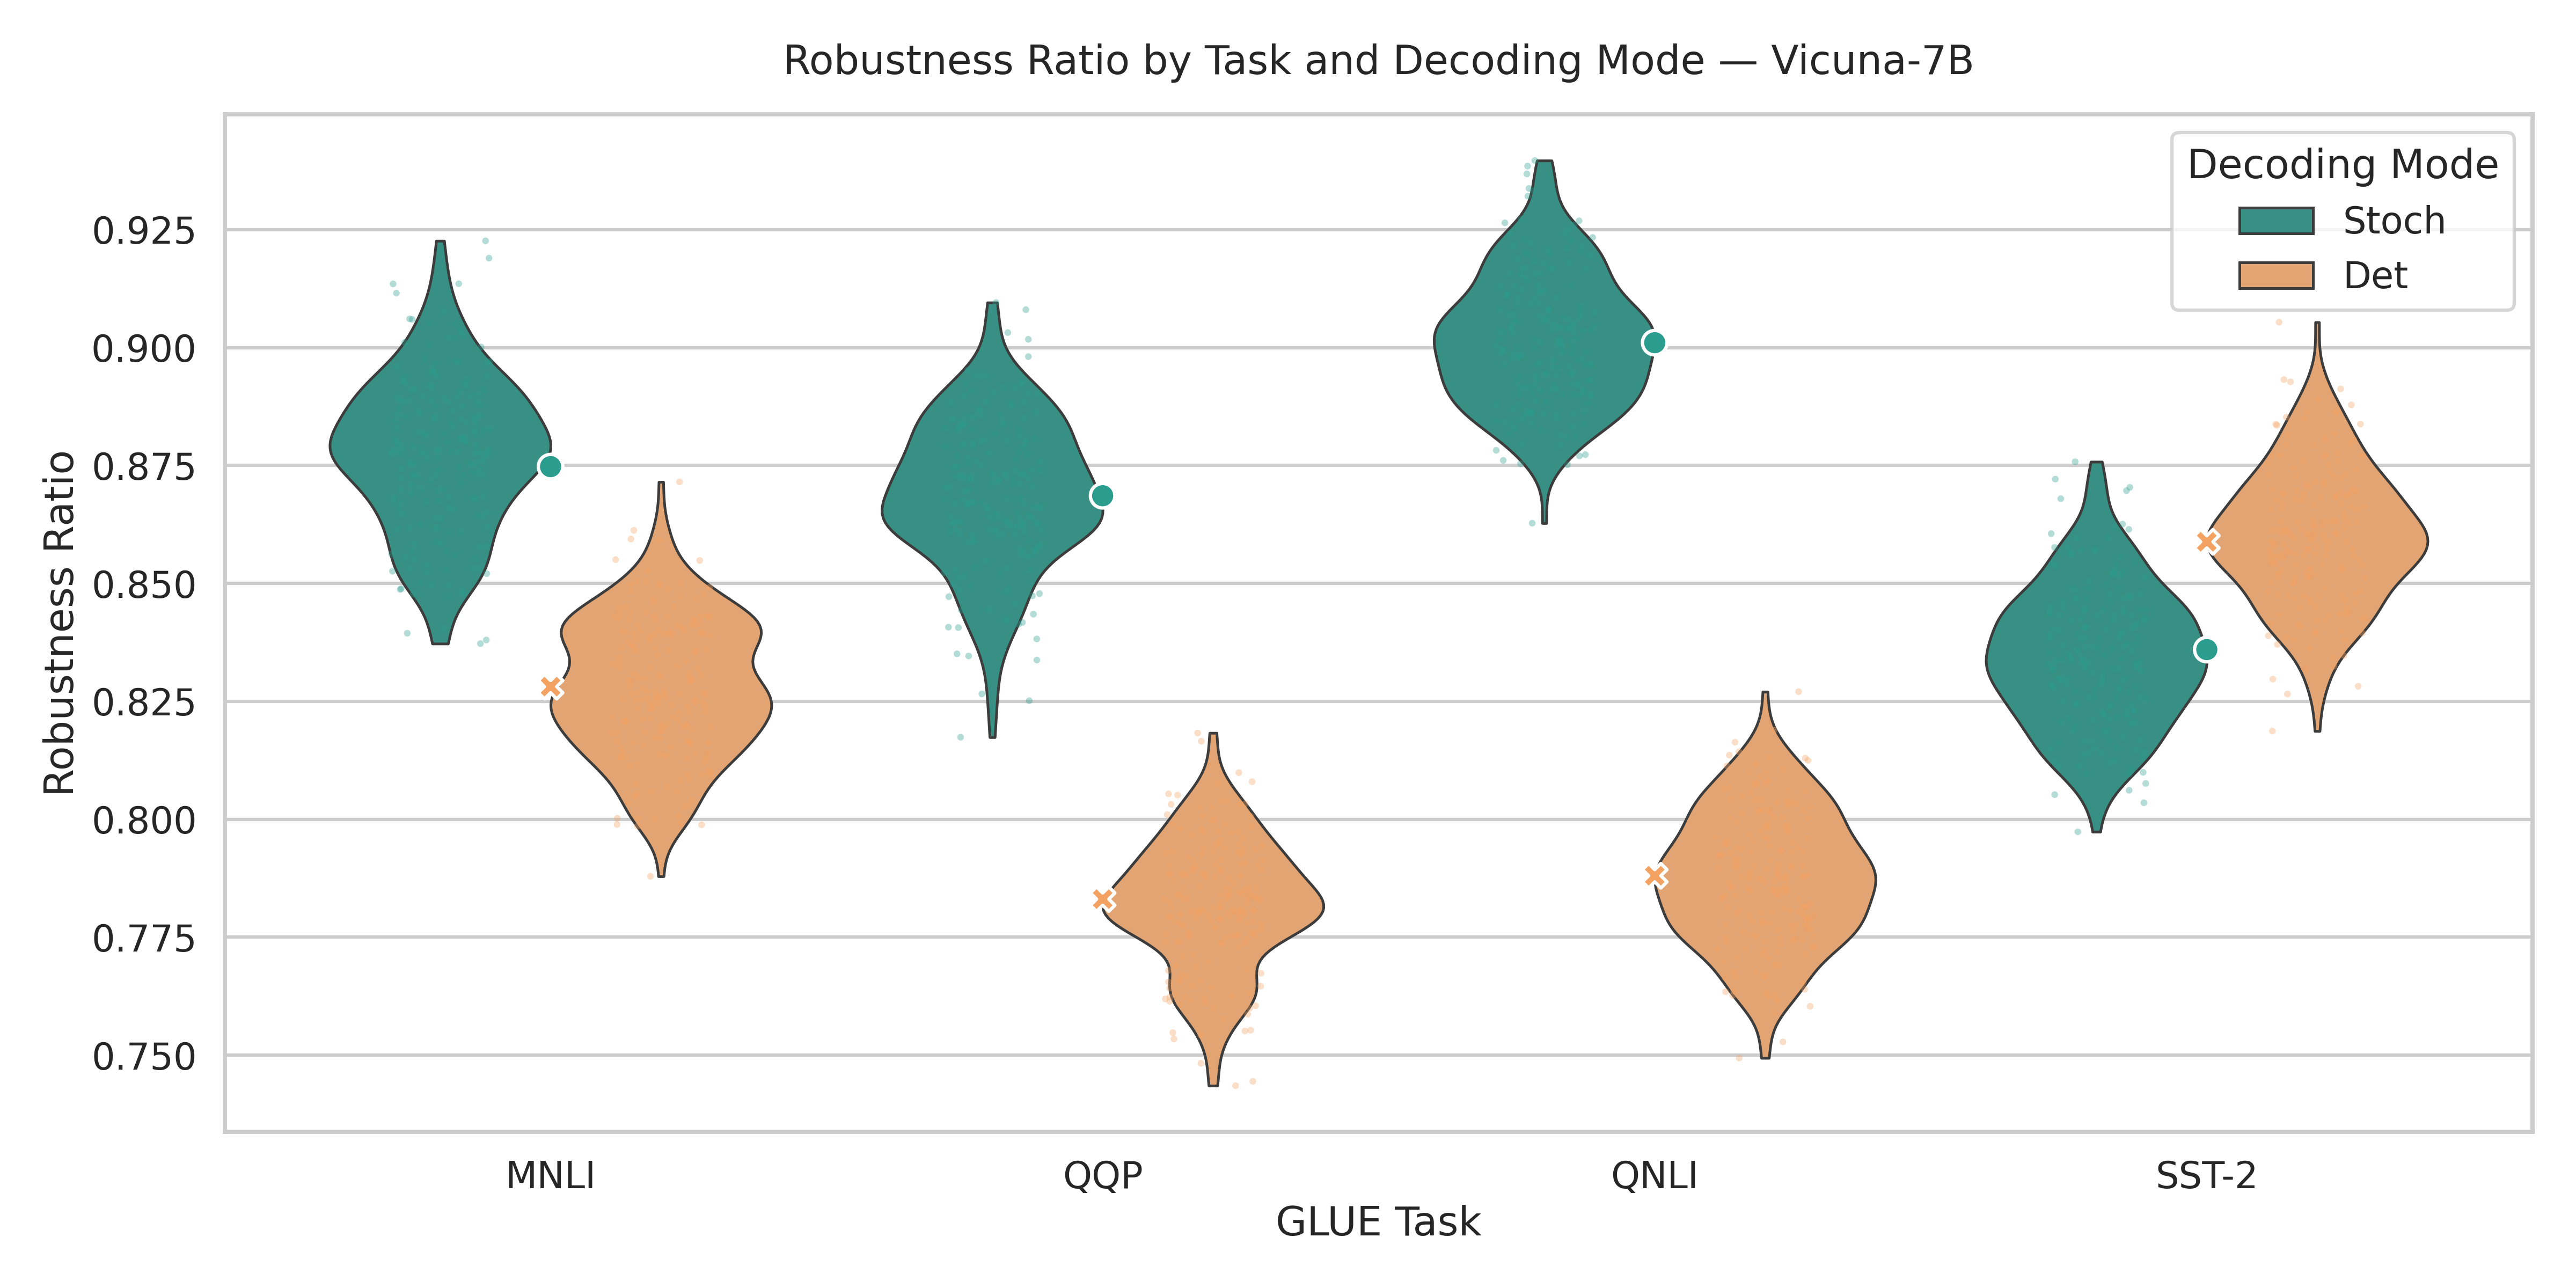
\includegraphics[width=\textwidth]{robustness_ratio/robustness_ratio_Vicuna-7B.png}
  \caption{
  \textbf{Robustness ratios for \emph{Vicuna-7B} across GLUE tasks.}
  With \textbf{stochastic decoding}, Vicuna-7B reaches robustness ratios of roughly \(\mathbf{0.88}\) on MNLI, \(\mathbf{0.87}\) on QQP, \(\mathbf{0.90}\) on QNLI, and \(\mathbf{0.82\text{--}0.84}\) on SST-2.
  \textbf{Deterministic decoding} lies around \(\mathbf{0.83}\) on MNLI, \(\mathbf{0.78}\) on QQP, \(\mathbf{0.79}\) on QNLI, and \(\mathbf{0.85\text{--}0.87}\) on SST-2.
  This produces positive stochastic–deterministic gaps of \(\mathbf{0.05\text{--}0.11}\) on MNLI/QQP/QNLI, but a \textbf{negative} gap on SST-2 where deterministic decoding is \(\approx\mathbf{0.03\text{--}0.04}\) higher.
  The figure thus reveals a \emph{\textbf{mixed robustness profile}}: Vicuna-7B strongly prefers stochastic decoding on inference-heavy tasks but appears better calibrated under deterministic decoding on sentiment classification.
  }
  \label{fig:robustness-vicuna7b}
\end{figure*}
